\chapter{DISEÑO DE CONTROL MIMO PID SINTETIZADO POR CONTROL LQI}
\label{cap:mimoPID} 
\renewcommand{\proofname}{Demostración}
\markboth{CAPÍTULO \thechapter. DISEÑO DE CONTROL MIMO PID}{CAPÍTULO \thechapter. DISEÑO DE CONTROL MIMO PID}

En este capítulo se desarrolla el diseño de control de la plataforma Stewart, caracterizado por ser un control MIMO PID sintetizado mediante un control LQI. Además, se desarrolla una versión descentralizada del controlador MIMO PID para ser optimizado mediante un algoritmo numérico. Los controladores desarrollados son simulados y comparados mediante tablas bajo distintos índices de desempeño.

%##############################################################
%##############################################################
\section{Diseño de controlador LQI para plataforma Stewart}
\lhead[\thepage]{Sección \thesection. Diseño control LQI}
\label{sec:lqi_stewart}

Se considera el sistema lineal transformado de la plataforma Stewart en \ref{eq:sys_varestados_transf}, con la diferencia de una matriz $C$ dada por $C_{pos}=\begin{bmatrix} I_{6\times6} & 0_{6\times6}\end{bmatrix}$. Esto quiere decir, que únicamente se tendrá como medición disponible del sistema las posiciones de los brazos, es decir, los primeros 6 estados internos de $\xi(t)$ mostrados en \ref{eq:sys_estados}. Además, se considera el diseño de control LQI presentado en el Capítulo \ref{cap:Notación y preliminares}. El diseño de control LQI se centrará en seguir a la referencia $r(t)$ definida únicamente con las posiciones deseadas de los brazos actuadores.  

Se define la ley de control para el estado aumentado $z(t)=\begin{bmatrix} \xi(t)^{\top} & \xi_{int}(t)^{\top} \end{bmatrix}^{\top}$ donde $\xi(t)$ son los estados internos del sistema lineal transformado denotados como $\xi(t) = \begin{bmatrix} l(t)^{\top} & \dot{l}(t)^{\top} \end{bmatrix}^{\top}$, y con $\xi_{int}(t)$ el nuevo estado definido como la integral del error de posición $\left(\xi_{int}(t)=\int r(t) - C_{pos} \xi(t)\right)$:

\begin{align}
    u^*(t) & = - K_z \cdot z(t) \notag \\
    & = -K_{pos} l(t) - K_{vel} \dot{l}(t) - K_{int} \xi_{int}(t)
\end{align}
donde $K_z = \begin{bmatrix} K_{pos} & K_{vel} & K_{int} \end{bmatrix}$ es la matriz de realimentación LQI.


%##############################################################
%##############################################################
\section{Diseño de controlador MIMO PID mediante control LQI}
\lhead[\thepage]{Sección \thesection. Diseño control MIMO PID}
\label{sec:mimopid_stewart}

Se considera el sistema lineal transformado de \ref{eq:sys_varestados_transf}, con su matriz $C$ original ($C_0$), es decir, con las salidas medibles disponibles de la posición y la velocidad de los brazos. 

Se posee una estructura general de un controlador PID, con las matrices $K_P$, $K_D$ y $K_I$ como las ganancias de proporcionalidad, derivativas y de integración respectivamente. 

Como la velocidad de la referencia es conocida, es posible desarrollar la actuación del sistema con el error de posición $ e(t) = r(t) - l(t)$ y el error de velocidad $\dot{e}(t) = \dot{r}(t) - \dot{l}(t)$

\begin{align} \label{eq:actuacion_pid}
    u(t) & = K_P e(t) + K_D \dot{e}(t) + K_I \frac{e(t)}{s} \notag \\
    & = K_P r(t) - K_P l(t) + K_D \dot{r}(t) - K_D \dot{l}(t) + K_I \frac{r(t)}{s} - K_I \frac{l(t)}{s}
\end{align}

De la sección anterior, se obtuvo la ley de control LQI dada por la actuación:
\begin{equation} \label{eq:actuacion_lqi}
    u(t) = -K_{pos} l(t) - K_{vel} \dot{l}(t) - K_{int} \frac{e(t)}{s}
\end{equation}

Comparando ambas actuaciones \ref{eq:actuacion_pid} y \ref{eq:actuacion_lqi}, se puede notar que para lograr una misma actuación, se necesita de un \textit{feedforward} en el controlador MIMO PID. El feedforward necesario para la actuación esta dado por $-K_P r(t) - K_D \dot{r}(t)$.

\begin{mybox}{}
    \begin{lemma} \label{lem4:mimo_pid}
        Se define el controlador MIMO PID con feedforward sintetizado por control LQI como:
        \begin{equation} \label{eq:actuacion_mimopid}
            u^*(t) = \left( K_P e(t) + K_D \dot{e}(t) + K_I \frac{e(t)}{s} \right) - K_P r(t) - K_D \dot{r}(t)
        \end{equation}
        
        con las ganancias $K_P$, $K_D$ y $K_I$ del controlador MIMO PID definidas por las ganancias de realimentación LQI $K_{pos}$, $K_{vel}$ y $K_{int}$:
        \begin{equation} \label{eq:gain_comparative_lqi_pid}
            K_P = K_{pos}, \qquad K_D = K_{vel}, \qquad K_I = -K_{int}
        \end{equation}
    \end{lemma}
\end{mybox}

En la Figura \ref{fig:pid_scheme} se ilustra el esquema de control MIMO PID con feedforward desarrollado.\\

Los controladores MIMO PID son poco comunes en la industria, y no es claro cuanto es la mejora real que pueden otorgar en comparación con los controladores PID descentralizados, los cuales son ampliamente usados. En las secciones siguientes se definirán controladores descentralizados para ser comparados con el MIMO PID desarrollado.

\begin{figure}[ht]
\centering
    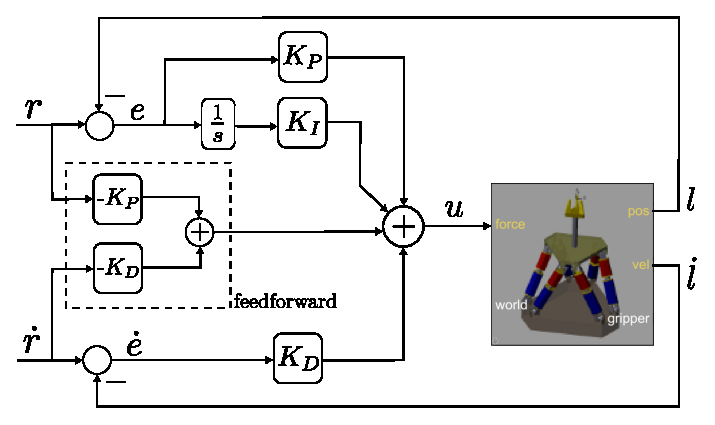
\includegraphics[width=0.7\columnwidth]{Figures/MIMO_PID/mimo_pid_scheme.eps}
    \caption{Esquema de control MIMO PID con feedforward para la plataforma Stewart.}
    \label{fig:pid_scheme}
\end{figure}

%##############################################################
%##############################################################
\section{Descentralización de controlador MIMO PID y optimización de desempeño}
\lhead[\thepage]{Sección \thesection. Diseño de control MIMO PID Descentralizado}
\label{sec:mimopid_descentralizado_stewart}

A partir del controlador MIMO PID obtenido anteriormente, se desarrolla la descentralización del PID junto a un algoritmo de optimización de desempeño, obteniéndose 2 tipos de controladores PID descentralizados para su posterior comparación con el controlador MIMO PID.

\subsection{Controlador PID descentralizado}

Considerando el controlador MIMO PID con feedforward de \ref{eq:actuacion_mimopid}, se define el controlador PID descentralizado con feedforward removiendo los términos fuera de la diagonal de las matrices $K_P$, $K_D$ y $K_I$, de la forma

\begin{equation} \label{eq:gain_lqi_desc}
    K_P^0 = K_P \odot I, \qquad K_D^0 = K_D \odot I, \qquad K_I^0 = K_I \odot I 
\end{equation}
donde $I$ es la matriz identidad y $\odot$ denota al producto de Hadamard.

\begin{remark}
    Se utiliza el sobrescrito $^0$ para representar las correspondientes matrices del controlador descentralizado inicial, diferenciándose con su versión descentralizada optimizada desarrollada a continuación con el sobrescrito $^N$, con $N$ el número de iteraciones del algoritmo de optimización.
\end{remark}

\subsection{Optimización PID descentralizado}

Para la optimización del controlador PID descentralizado obtenido anteriormente, se utiliza un algoritmo numérico de \cite{silva2006lqr}. Este algoritmo emplea como técnica un simple descenso del gradiente que converge iterativamente en una solución descentralizada óptima para problemas de control LQR.

Para nuestro caso, se contempla el sistema aumentado \ref{eq:sys_aumentado_lqi} con el sistema lineal transformado \ref{eq:sys_varestados_transf} de la plataforma Stewart utilizado en el diseño de control LQI. Además se considera la matriz de realimentación LQI descentralizada con las ganancias obtenidas en \ref{eq:gain_lqi_desc}:
\begin{equation} \label{eq:gain_lqi_desc2}
    K_z^0 = \begin{bmatrix}
        K_P^0 & K_D^0 & -K_I^0
    \end{bmatrix}
\end{equation}
para la ley de control 
\begin{equation}
    u(t) = -K_z^0 \cdot z(t)
\end{equation}
con $z(t)=\begin{bmatrix} \xi(t)^{\top} & \xi_{int}(t)^{\top} \end{bmatrix}^{\top} = \begin{bmatrix} l(t)^{\top} & \dot{l}(t)^{\top} & \xi_{int}(t)^{\top} \end{bmatrix}^{\top}$ el estado aumentado del sistema.

Se deduce que la función objetivo LQR promediada del estado inicial estándar se puede escribir como:

\begin{equation}
    J(K) = \textrm{trace} \left\{ F(K) \right\}
\end{equation}
donde $F(K)$ es la función de coste LQR de la forma:
\begin{equation} \label{eq:costo_algorithm_F(K)}
    F(K) = \int_0^\infty \Lambda(t)^{\top} \left( \Psi + K^{\top} \Omega K \right) \Lambda(t) \quad dt
\end{equation}

con $\Lambda(t) = e^{(A_a+B_a K)t}$, $\Psi \geq 0$ y $\Omega > 0$. Se debe notar que como $A_a + B_a K$ es estable, es posible obtener $F(K)$ de otra forma, como la solución a la ecuación de Lyapunov siguiente:

\begin{equation} \label{eq:algorithm_F(K)}
    \left( A_a + B_a K \right)^{\top} F(K) + F(K) \left( A_a + B_a K \right) + \left( \Psi + K^{\top} \Omega K \right) = 0
\end{equation}

Se inicia con una solución estable dada por $K = K_0$ (en nuestro caso la solución inicial será $K_z^0$ definida en \ref{eq:gain_lqi_desc2}), para descender en dirección contraria al gradiente disminuyendo el valor del funcional de costo de la forma $K=K_0-\textit{dirección-contragradiente}$. Para esto se define el $i^{th}$ candidato $K$, tal que $K_i$:

\begin{equation}
    K_i = K_{i-1} - \mu \frac{d}{dK}\textrm{ trace}\left\{ F(K_{i-1}) \right\} \qquad i = 1,2,\hdots,N
\end{equation}

donde $N$ es el número de iteraciones y $\mu>0$ es un número real pequeño relacionado con la velocidad de convergencia y estabilidad del algoritmo. Es posible escribir la derivada de la traza como: 

\begin{equation}
    \frac{d}{dK} \textrm{ trace} \left\{F(K_i)\right\} = 2\left( \Omega K_i + B_a^{\top} F(K_i) \right) W
\end{equation}
con $F(K_i)$ definido en \ref{eq:costo_algorithm_F(K)} y \ref{eq:algorithm_F(K)}, y con $W$ la solución a la ecuación de Lyapunov:
\begin{equation}
    \left( A_a + B_a K_i \right) W + W \left( A_a + B_a K_i \right)^{\top} + I = 0
\end{equation}
con I la matriz identidad.

Es posible que el gradiente de $K=K_{i-1}$ no posea necesariamente la estructura deseada de la solución que se busca, ya que a medida que se desarrollan las iteraciones buscando un óptimo, puede que la estructura se pierda. Para prevenir esto se establece un operador $\textrm{sp}\{\cdot\}$ encargado de conservar la estructura deseada, que en nuestro caso se basa en diagonalizar el gradiente, para así mantener la estructura descentralizada que se busca. Dada una matriz $X$ se define el operador $\textrm{sp}\{\cdot\}$:

\begin{equation}
    \textrm{sp} \left\{ X \right\} = X \odot \begin{bmatrix}
        I & I & I
    \end{bmatrix}
\end{equation}

con $I$ matrices identidad de dimensiones apropiadas. De esta forma es posible actualizar la ecuación de optimización descentralizada como:

\begin{equation}
    K_i = K_{i-1} - \mu \textrm{ sp} \left\{\frac{d}{dK}\textrm{ trace}\left\{ F(K_{i-1}) \right\} \right\} 
\end{equation}

El algoritmo descrito preserva la estructura deseada del controlador en cada iteración, pero la estabilidad del mismo puede perderse. Para solucionar esto, se debe verificar la estabilidad del controlador previo a cada actualización, descartando los controladores $K_i$ que no son estables. Escogiendo un valor de $\mu$ suficientemente pequeño se garantiza no perder estabilidad en el controlador iterado.



%##############################################################
%##############################################################
\newpage
\section{Resultados de simulación MIMO PID}
\lhead[\thepage]{Sección \thesection. Resultados de simulación MIMO PID}
\label{sec:resultados_mimoPID}

Los resultados de los distintos controladores son comparados mediante índices de desempeño en tablas comparativas. Estos índices de desempeño se definen como la integral del error cuadrático ($J_{ISE}$), el esfuerzo de control definido por la integral de la actuación cuadrática ($J_u$), y la función de costo LQI ($J_{LQI}$). Se muestra a continuación la definición de los respectivos índices de desempeño:
\begin{align} \label{eq:indices_desempeño}   
    J_{ISE} & = \int_0^{T_{sim}} e(t)^\top e(t) dt, \\ 
    J_{u} & = \int_0^{T_{sim}} u(t)^\top u(t) dt,\\
    J_{LQI} & =\int_0^{T_{sim}} \left( z(t)^{\top}Qz(t) + u(t)^{\top}Ru(t) \right) \ dt
\end{align}
con $T_{sim}$ el tiempo de simulación y $z(t)=\begin{bmatrix} \xi(t)^{\top} & \xi_i(t)^{\top} \end{bmatrix}^{\top}$ el estado aumentado. Se debe destacar que se utiliza $S=0$ para la función de coste genérica LQI descrita en el capítulo \ref{cap:Notación y preliminares}, obteniendo así el coste $J_{LQI}$ recién mencionado.

Se establecen 2 casos a estudiar, para distintos valores de las matrices $Q$ y $R$ en la obtención de la matriz de realimentación LQI para el diseño de control MIMO PID. La matriz de realimentación se obtiene mediante el comando \textit{lqi()} con el sistema lineal transformado \ref{eq:sys_varestados_transf} y $C_{pos}$, definido en la sección \ref{sec:lqi_stewart}.

En todos los casos estudiados, los parámetros del algoritmo de optimización utilizados para el controlador descentralizado son $\mu=5\cdot 10^{-4}$ y $N=1000$ iteraciones para la tasa de convergencia. Mediante experimentación se encontró que estos valores son suficientes para observar una convergencia en el algoritmo de optimización.

\subsubsection{Caso 1:}
Para el Caso 1 los parámetros en la obtención de la matriz de realimentación LQI son:
\begin{equation}
    Q = I_{18\times18}, \qquad R = 0.1\cdot I_{6\times6}
\end{equation}
con $I$ la matriz identidad. La matriz $Q$ identidad pondera a todos los estados por igual. Por otro lado con la matriz $R$ se penaliza levemente la actuación de entrada para así no restringir tanto su efecto en el sistema.

Las matrices del controlador MIMO PID sintetizadas por diseño de control LQI en la sección \ref{sec:mimopid_stewart} son:

\begin{equation}
    K_P = \begin{bmatrix}
        15.164&	\textrm{-}6.499&	\textrm{-}2.054&	4.022&	\textrm{-}1.492&	\textrm{-}3.397 \\
        \textrm{-}6.506&	15.134&	\textrm{-}3.391&	\textrm{-}1.473&	4.016&	\textrm{-}2.036 \\
        \textrm{-}1.471&	\textrm{-}3.436&	15.206&	\textrm{-}6.506&	\textrm{-}2.052&	4.017 \\
        3.994&	\textrm{-}2.072&	\textrm{-}6.496&	15.222&	\textrm{-}3.443&	\textrm{-}1.465 \\
        \textrm{-}2.100&	3.975&	\textrm{-}1.447&	\textrm{-}3.434&	15.232&	\textrm{-}6.485 \\
        \textrm{-}3.423&	\textrm{-}1.451&	4.009&	\textrm{-}2.053&	\textrm{-}6.515&	15.191 \\
    \end{bmatrix}
\end{equation}

\begin{equation}
    K_D = \begin{bmatrix}
        3.890&	\textrm{-}0.567&	\textrm{-}0.279&	0.395&	\textrm{-}0.133&	\textrm{-}0.072 \\
        \textrm{-}0.565&	3.888&	\textrm{-}0.073&	\textrm{-}0.132&	0.394&	\textrm{-}0.278 \\
        \textrm{-}0.132&	\textrm{-}0.073&	3.891&	\textrm{-}0.567&	\textrm{-}0.279&	0.396 \\
        0.396&	\textrm{-}0.280&	\textrm{-}0.568&	3.892&	\textrm{-}0.074&	\textrm{-}0.132 \\
        \textrm{-}0.281&	0.397&	\textrm{-}0.131&	\textrm{-}0.074&	3.893&	\textrm{-}0.568 \\
        \textrm{-}0.074&	\textrm{-}0.132&	0.396&	\textrm{-}0.279&	\textrm{-}0.567&	3.890 \\
    \end{bmatrix}
\end{equation}

\begin{equation}
    K_I = -\begin{bmatrix}
	\textrm{-}3.159&	0.0008&	0.096&	0.0007&	\textrm{-}0.100&	\textrm{-}0.0008 \\
	\textrm{-}0.0009&	\textrm{-}3.159&	\textrm{-}1.64\cdot10^{\textrm{-}5}&	\textrm{-}0.100&	0.001& 0.096 \\
	\textrm{-}0.099&	0.0001&	\textrm{-}3.159&	\textrm{-}0.0004&	0.097&	9.11\cdot10^{\textrm{-}5} \\
	\textrm{-}0.0006&	0.097&	0.0004&	\textrm{-}3.159&	\textrm{-}0.0004&	\textrm{-}0.100 \\
	0.097&	\textrm{-}0.001&	\textrm{-}0.100&	0.0003&	\textrm{-}3.159&	0.001 \\
	0.0008&	\textrm{-}0.099&	\textrm{-}0.0001&	0.097&	\textrm{-}0.0009&	\textrm{-}3.159 \\
    \end{bmatrix}
\end{equation}

Las matrices del controlador MIMO PID Descentralizado de la sección \ref{sec:mimopid_descentralizado_stewart} para el Caso 1 son:

\begin{equation}
    K_P^0 = K_P \odot I, \qquad K_D^0 = K_D \odot I, \qquad K_I^0 = K_I \odot I
\end{equation}
donde $I$ es la matriz identidad y $\odot$ el producto de Hadamard.

Las matrices del Caso 1 para el controlador MIMO PID Descentralizado Optimizado mediante el algoritmo de optimización con 1000 iteraciones, mencionado en la sección \ref{sec:mimopid_descentralizado_stewart}, son:

\begin{equation}
    K_P^{1000} = \begin{bmatrix}
        15.0839 &	0 &	0 &	0 &	0 &	0 \\
        0 &	15.0540 &	0 &	0 &	0 &	0 \\
        0 &	0 &	15.1259 &	0 &	0 &	0 \\
        0 &	0 &	0 &	15.1423 &	0 &	0 \\
        0 &	0 &	0 &	0 &	15.1514 &	0 \\
        0 &	0 &	0 &	0 &	0 &	15.1113 \\
    \end{bmatrix}
\end{equation}

\begin{equation}
    K_D^{1000} = \begin{bmatrix}
        4.0673 &	0 &	0 &	0 &	0 &	0 \\
        0 &	4.0653 &	0 &	0 &	0 &	0 \\
        0 &	0 &	4.0693 &	0 &	0 &	0 \\
        0 &	0 &	0 &	4.0702 &	0 &	0 \\
        0 &	0 &	0 &	0 &	4.0708 &	0 \\
        0 &	0 &	0 &	0 &	0 &	4.0685 \\
    \end{bmatrix}
\end{equation}

\begin{equation}
    K_I^{1000} = -\begin{bmatrix}
    \textrm{-}3.5441 &	0 &	0 &	0 &	0 &	0 \\
    0 &	\textrm{-}3.5434 &	0 &	0 &	0 &	0 \\
    0 &	0 &	\textrm{-}3.5459 &	0 &	0 &	0 \\
    0 &	0 &	0 &	\textrm{-}3.5459 &	0 &	0 \\
    0 &	0 &	0 &	0 &	\textrm{-}3.5458 &	0 \\
    0 &	0 &	0 &	0 &	0 &	\textrm{-}3.5454 \\
    \end{bmatrix}
\end{equation}

\subsubsection{Caso 2:}
Para el Caso 2 los parámetros en la obtención de la matriz de realimentación LQI son:
\begin{equation}
    Q = \begin{bmatrix} C_0^\top C_0 & 0 \\ 0 & 100\cdot I_{6\times6} \end{bmatrix}, \qquad R = 0.1\cdot I_{6\times6} 
\end{equation}
con $C_0$ la matriz de salida del sistema linealizado transformado \ref{eq:sys_varestados_transf} e $I$ la matriz identidad. En este caso, en la matriz $Q$ los estados correspondientes a la integral del error son ponderados en mayor medida que los demás, para así darle más importancia al seguimiento de la referencia. Por otro lado, con la matriz $R$ bajamente ponderada, no se castiga en gran cantidad la actuación para así no restringir su efecto en el sistema.

Las matrices del controlador MIMO PID sintetizadas por diseño de control LQI en la sección \ref{sec:mimopid_stewart} son:

\begin{equation} \label{eq:KP_mimoPID}
    K_P = \begin{bmatrix}
        24.037 &	\textrm{-}6.357 &	\textrm{-}2.141 &	3.812 &	\textrm{-}1.493 &	\textrm{-}2.746 \\
        \textrm{-}6.363 &	24.013 &	\textrm{-}2.739 &	\textrm{-}1.479 &	3.807 &	\textrm{-}2.125 \\
        \textrm{-}1.478 &	\textrm{-}2.785 &	24.078 &	\textrm{-}6.361 &	\textrm{-}2.137 &	3.807 \\
        3.784 &	\textrm{-}2.159 &	\textrm{-}6.351 &	24.089 &	\textrm{-}2.786 &	\textrm{-}1.467 \\
        \textrm{-}2.181 &	3.768 &	\textrm{-}1.452 &	\textrm{-}2.777 &	24.093 &	\textrm{-}6.341 \\
        \textrm{-}2.773 &	\textrm{-}1.461 &	3.799 &	\textrm{-}2.136 &	\textrm{-}6.370 &	24.065 \\
    \end{bmatrix}
\end{equation}

\begin{equation} \label{eq:KD_mimoPID}
    K_D = \begin{bmatrix}
        4.150 &	\textrm{-}0.710 &	\textrm{-}0.304 &	0.443 &	\textrm{-}0.194 &	\textrm{-}0.038 \\
        \textrm{-}0.709 &	4.148 &	\textrm{-}0.038 &	\textrm{-}0.193 &	0.442 &	\textrm{-}0.303 \\
        \textrm{-}0.193 &	\textrm{-}0.038 &	4.158 &	\textrm{-}0.710 &	\textrm{-}0.304 &	0.443 \\
        0.444 &	\textrm{-}0.305 &	\textrm{-}0.711 &	4.151 &	\textrm{-}0.039 &	\textrm{-}0.193 \\
        \textrm{-}0.306 &	0.445 &	\textrm{-}0.192 &	\textrm{-}0.040 &	4.152 &	\textrm{-}0.711 \\
        \textrm{-}0.039 &	\textrm{-}0.192 &	0.443 &	\textrm{-}0.304 &	\textrm{-}0.710 &	4.150 \\
    \end{bmatrix}
\end{equation}

\begin{equation} \label{eq:KI_mimoPID}
    K_I = -\begin{bmatrix}
    	\textrm{-}31.611 &	0.005 &	0.577 &	0.004 &	\textrm{-}0.594 &	\textrm{-}0.005 \\
    	\textrm{-}0.005 &	\textrm{-}31.611 &	\textrm{-}0.0002 &	\textrm{-}0.594 & 0.012 & 0.576 \\
    	\textrm{-}0.588 &	0.0006 &	\textrm{-}31.611 &	\textrm{-}0.002 &	0.582 &	0.0005 \\
    	\textrm{-}0.004 &	0.584 &	0.002 &	\textrm{-}31.611 &	\textrm{-}0.002 &	\textrm{-}0.592 \\
    	0.583 &	\textrm{-}0.012 &	\textrm{-}0.593 &	0.002 &	\textrm{-}31.611 &	0.005 \\
    	0.005 &	\textrm{-}0.587 &	\textrm{-}0.0008 &	0.581 &	\textrm{-}0.005 &	\textrm{-}31.611 \\
    \end{bmatrix}
\end{equation}

Las matrices del controlador MIMO PID Descentralizado de la sección \ref{sec:mimopid_descentralizado_stewart} para el Caso 2 son:

\begin{equation}
    K_P^0 = K_P \odot I, \qquad K_D^0 = K_D \odot I, \qquad K_I^0 = K_I \odot I
\end{equation}
donde $I$ es la matriz identidad y $\odot$ el producto de Hadamard.

Las matrices del Caso 2 para el controlador MIMO PID Descentralizado Optimizado mediante el algoritmo de optimización con 1000 iteraciones, mencionado en la sección \ref{sec:mimopid_descentralizado_stewart}, son:

\begin{equation}
    K_P^{1000} = \begin{bmatrix}
        23.5097 &	0 &	0 &	0 &	0 &	0 \\
        0 &	23.4860 &	0 &	0 &	0 &	0 \\
        0 &	0 &	23.5490 &	0 &	0 &	0 \\
        0 &	0 &	0 &	23.5603 &	0 &	0 \\
        0 &	0 &	0 &	0 &	23.5639 &	0 \\
        0 &	0 &	0 &	0 &	0 &	23.5361 \\
    \end{bmatrix}
\end{equation}

\begin{equation}
    K_D^{1000} = \begin{bmatrix}
        3.7832 &	0 &	0 &	0 &	0 &	0 \\
        0 &	3.7813 &	0 &	0 &	0 &	0 \\
        0 &	0 &	3.7857 &	0 &	0 &	0 \\
        0 &	0 &	0 &	3.7866 &	0 &	0 \\
        0 &	0 &	0 &	0 &	3.7869 &	0 \\
        0 &	0 &	0 &	0 &	0 &	3.7848 \\
    \end{bmatrix}
\end{equation}

\begin{equation}
    K_I^{1000} = -\begin{bmatrix}
        \textrm{-}32.1930 &	0 &	0 &	0 &	0 &	0 \\
        0 &	\textrm{-}32.1922 &	0 &	0 &	0 &	0 \\
        0 &	0 &	\textrm{-}32.1953 &	0 &	0 &	0 \\
        0 &	0 &	0 &	\textrm{-}32.1952 &	0 &	0 \\
        0 &	0 &	0 &	0 &	\textrm{-}32.1950 &	0 \\
        0 &	0 &	0 &	0 &	0 &	\textrm{-}32.1948 \\
    \end{bmatrix}
\end{equation}



%%%%%%%%%%%%%%%%%%%%%%%%%%%%%%%%%%%%%%%%%%%%%%%%
\subsection{Referencia Escalón}

Se establece la señal de referencia para el movimiento de la plataforma superior por señales tipo escalón, donde en este caso describe un largo constante de brazos brindando una elevación fija a la plataforma superior:
\begin{equation} 
    q_{ref} = \begin{bmatrix}
        0 & 0 & 14 & 0 & 0 & 0
    \end{bmatrix}^{\top}
\end{equation}

Para un tiempo de simulación de $T_{sim}=50(s)$ se obtienen los resultados de los índices de desempeño mostrados en la tabla comparativa \ref{tab:indices_mimopid_escalon}:

\begin{table}[ht]
\centering
\begin{tabular}{c|c|c|c|c|}
\cline{2-5}
    & \textbf{PID MIMO} & $\mathbf{J_{ISE}}$ & $\mathbf{J_{u}}(\cdot10^5)$ & $\mathbf{J_{LQI}}(\cdot10^6)$ \\ \hline
\multicolumn{1}{|c|}{\multirow{3}{*}{Caso 1}} &  Full               & $2166$  & $3.5864$  & $0.4156$ \\ \cline{2-5} 
\multicolumn{1}{|c|}{}                        & Descentralizado 0   & $3367$  & $3.6082$  & $1.4256$ \\ \cline{2-5} 
\multicolumn{1}{|c|}{}                        & Descentralizado 1000& $3003$  & $3.6031$  & $1.1596$ \\ \hline
\multicolumn{1}{|c|}{\multirow{3}{*}{Caso 2}} & Full                & $399.1$ & $3.5660$  & $1.6167$ \\ \cline{2-5} 
\multicolumn{1}{|c|}{}                        & Descentralizado 0   & $516.6$ & $3.5687$  & $3.5093$ \\ \cline{2-5} 
\multicolumn{1}{|c|}{}                        & Descentralizado 1000& $496.9$ & $3.5687$  & $3.2593$ \\ \hline
\end{tabular}
\caption{Desempeño para PID MIMO Full y PID MIMO Descentralizado con $N=0$ y $N=1000$ iteraciones, referencia escalón.}
\label{tab:indices_mimopid_escalon}
\end{table}

Como se puede apreciar de la tabla \ref{tab:indices_mimopid_escalon} comparativa, para ambos casos se aprecia que el controlador MIMO PID Full posee los índices del error cuadrático ($J_{ISE}$) más bajos que los demás, siendo así mejores. Si usamos los índices del controlador MIMO PID Full como referencia, el controlador MIMO PID Descentralizado 0 muestra un $55.4\%$ de incremento del $J_{ISE}$ para el Caso 1 y un $29.4\%$ para el Caso 2. Siguiendo esta misma lógica, el controlador optimizado MIMO PID Descentralizado 1000 posee un incremento del $38.6\%$ para el Caso 1 y un $24.5\%$ para el Caso 2 del índice $J_{ISE}$, evidenciándose la mejoría del algoritmo de optimización al bajar el índice $J_{ISE}$ pero aun así sin poder igualar al MIMO PID Full.

Por otro lado, los valores del esfuerzo de control ($J_u$) son altos para ambos casos en todos los controladores. Tomando el controlador MIMO PID Full como referencia, el controlador MIMO PID Descentralizado 0 posee un aumento del $0.6\%$ para el Caso 1 y un $0.07\%$ para el Caso 2 en el índice $J_{u}$. Para el controlador optimizado MIMO PID Descentralizado 1000 este posee un $0.4\%$ en el Caso 1 y un $0.07\%$ para el Caso 2. Esta pequeña diferencia nos demuestra que el esfuerzo de control es casi el mismo para los 3 tipos de controladores, pero si se busca escoger el mejor sigue siendo el controlador MIMO PID Full.

Finalmente el índice de la función de coste LQI ($J_{LQI}$) muestra que el controlador MIMO PID Full es mejor que los demás al poseer los valores más pequeños de este índice. Al tomar este controlador MIMO PID Full como referencia para el índice $J_{LQI}$, podemos ver que la versión MIMO PID Descentralizado 0 posee un incremento del $243\%$ para el caso 1 y un $117\%$ para el Caso 2. Por otro lado el controlador optimizado MIMO PID Descentralizado 1000 posee un aumento del $179\%$ para el caso 1 y un $101.6\%$ para el Caso 2. 

Con esto, se demuestra la eficacia y el mejor desempeño en todos los ámbitos anteriores del controlador MIMO PID Full en comparación a sus versiones descentralizadas. 

En las Figuras \ref{fig:result_mimoPID_escalon_error1} y \ref{fig:result_mimoPID_escalon_fuerza1} se muestra el error de seguimiento y la fuerza aplicada respectivamente en cada brazo de la plataforma Stewart para el Caso 1. Se demuestra que el controlador MIMO PID Full posee un correcto seguimiento de la referencia, garantizando un error cero de seguimiento en estado estacionario. Sin embargo, las versiones descentralizadas comienzan a desestabilizarse a partir de los 30 segundos, apreciándose claramente en las gráficas de las fuerzas de los brazos. 

Con esto podemos deducir que para el Caso 1 las matrices $Q$ y $R$ escogidas nos limitan la velocidad de control, repercutiendo en que los controladores descentralizados no son capaces de estabilizar el sistema, siendo necesaria la versión MIMO PID Full para lograr un correcto control para la referencia tipo escalón. 
 
\begin{figure}[H]
\centering
    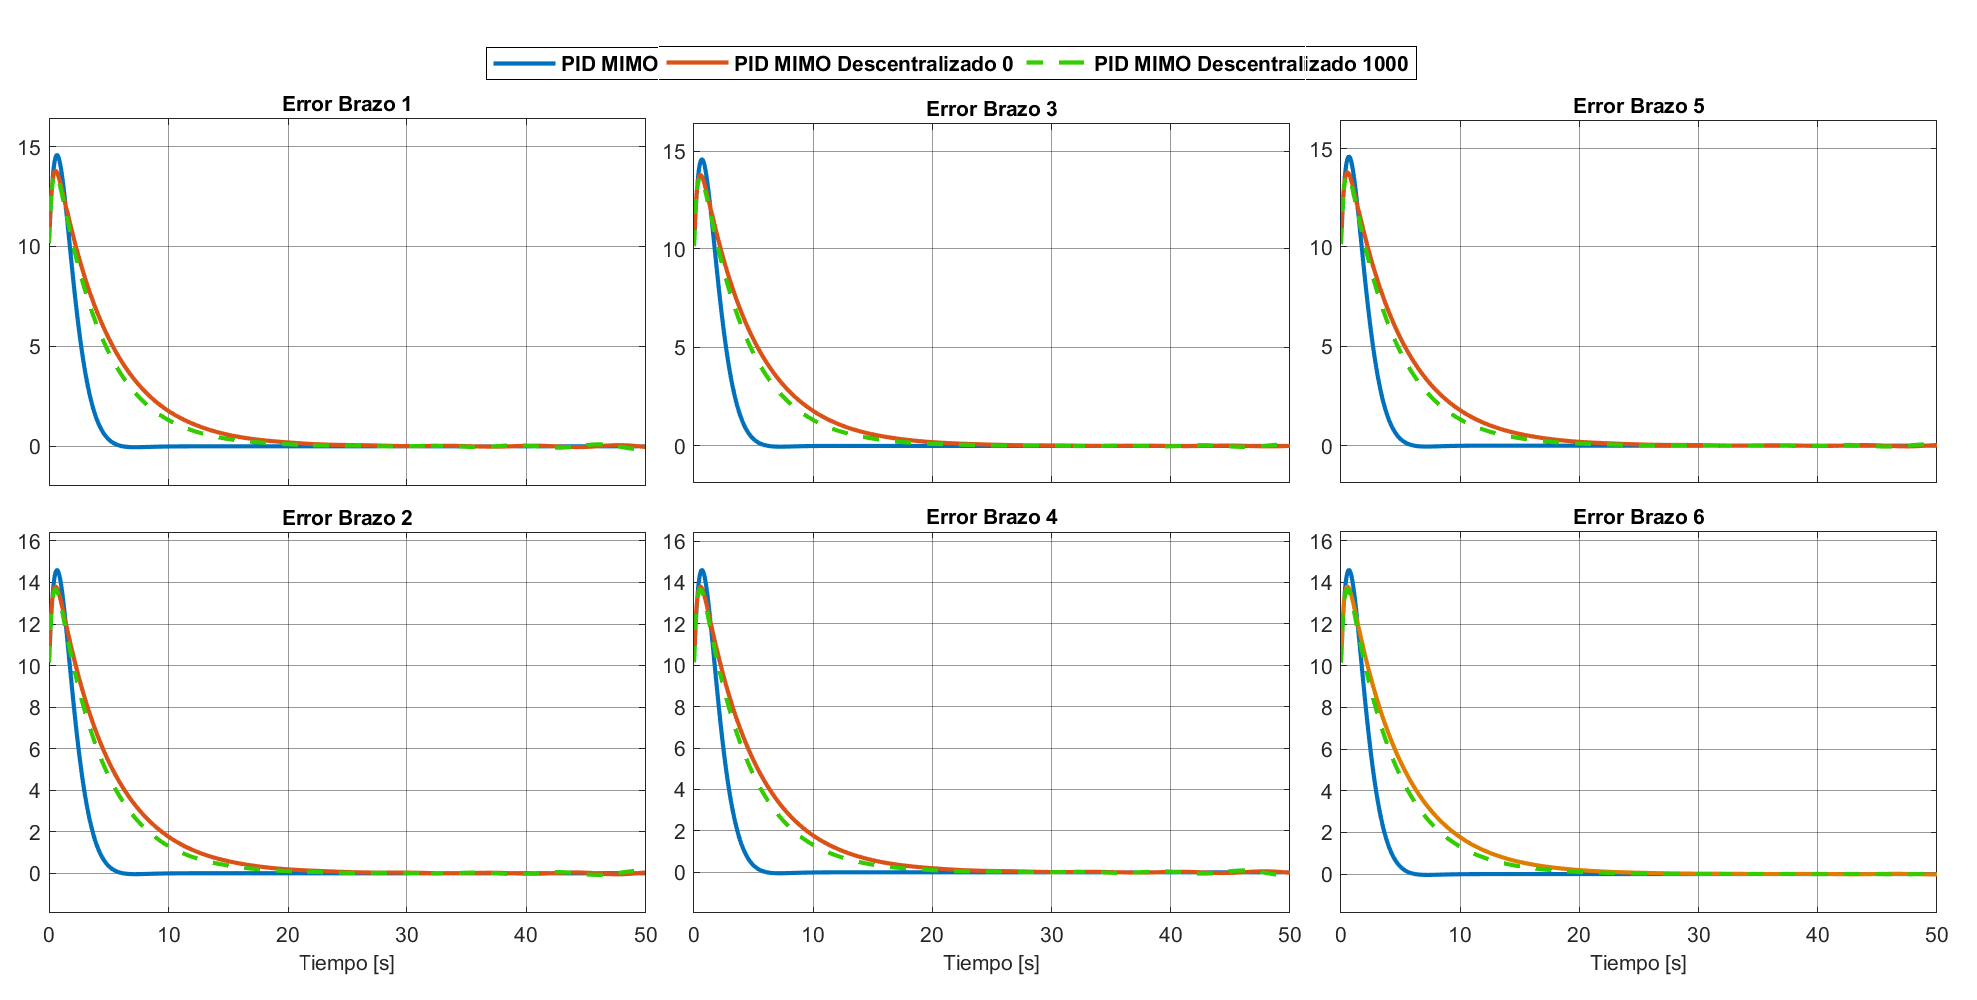
\includegraphics[width=1\columnwidth]{Results/mimoPID_escalon/CASO_1_error_escalon.eps}
    \caption{CASO 1 Error de seguimiento (cm), referencia escalón.}
    \label{fig:result_mimoPID_escalon_error1}
\end{figure}
\newpage
\begin{figure}[H]
\centering
    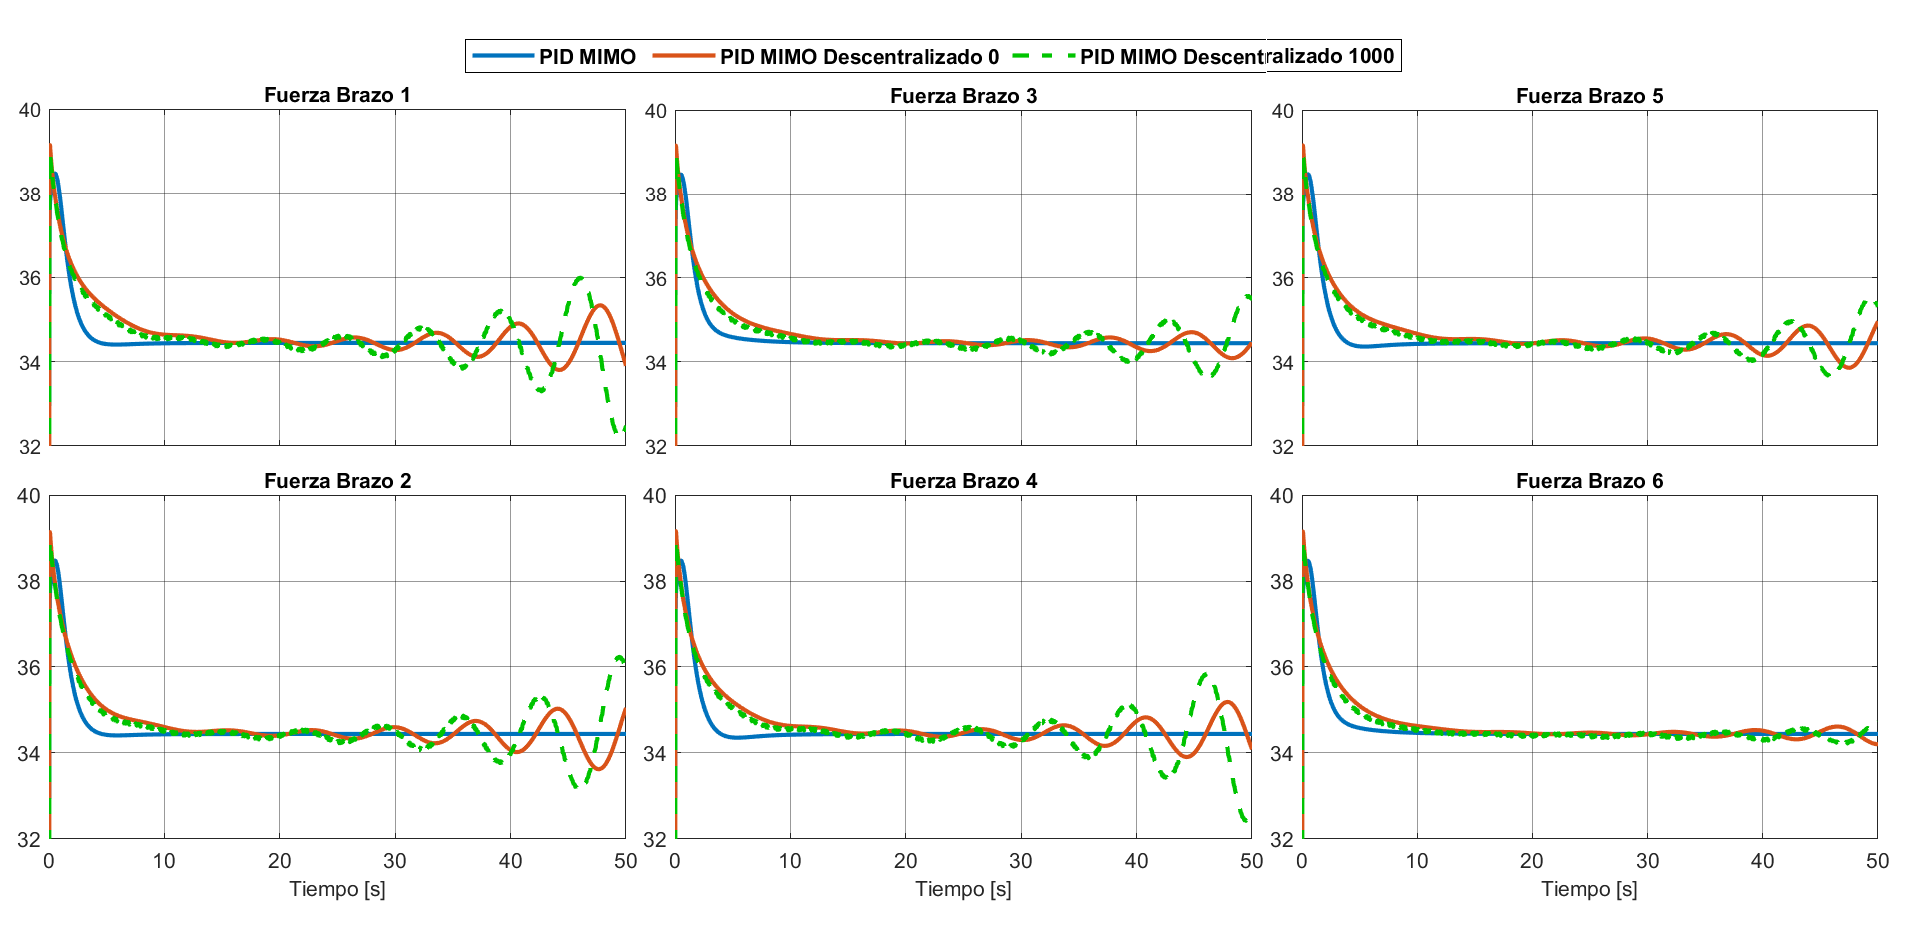
\includegraphics[width=1\columnwidth]{Results/mimoPID_escalon/CASO_1_fuerza_escalon.eps}
    \caption{CASO 1 Fuerza de actuación (N), referencia escalón.}
    \label{fig:result_mimoPID_escalon_fuerza1}
\end{figure}

Para el caso 2, el cambio de las matrices $Q$ y $R$ se traduce en una respuesta más rápida del control, disminuyendo considerablemente el transciente del error y de la fuerza. En las Figuras \ref{fig:result_mimoPID_escalon_error2} y \ref{fig:result_mimoPID_escalon_fuerza2} se muestra el error de seguimiento y la fuerza aplicada respectivamente en cada brazo de la plataforma Stewart. Los 3 tipos de controladores son capaces de estabilizar la plataforma, garantizando un error cero en estado estacionario. 

\begin{figure}[H]
\centering
    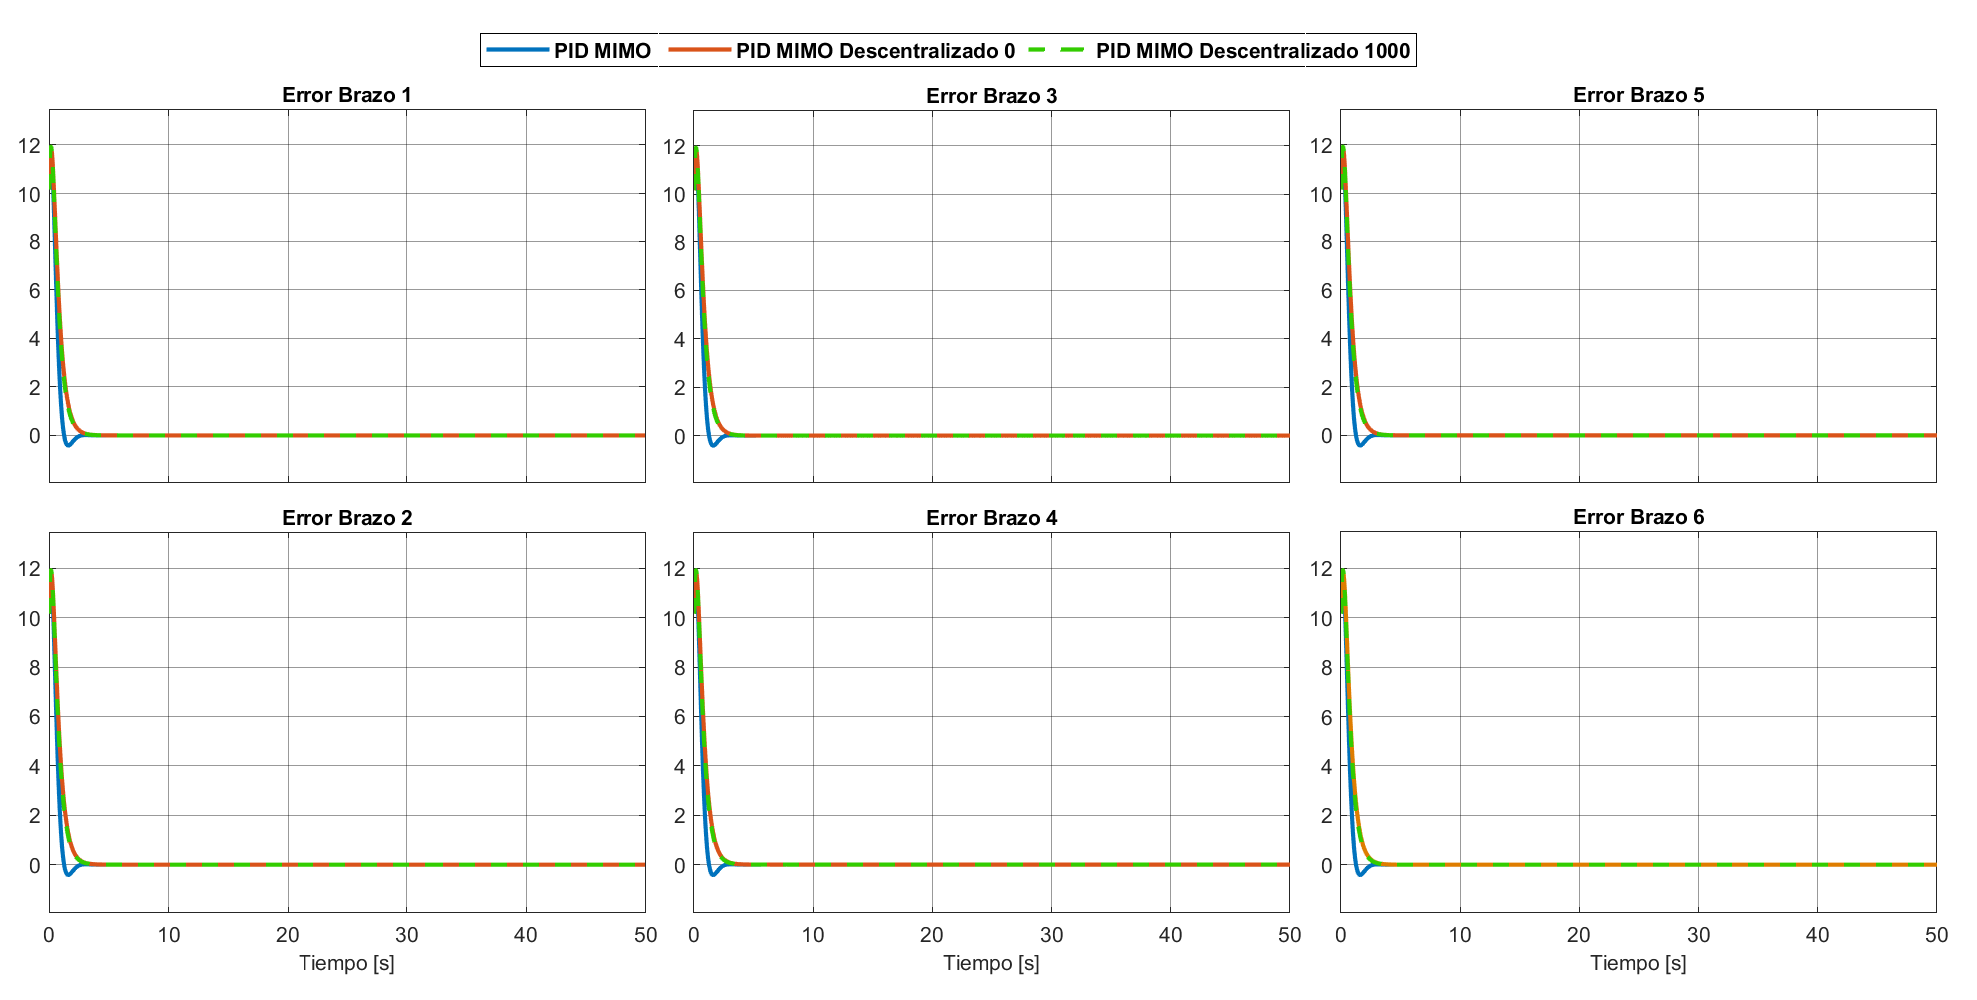
\includegraphics[width=1\columnwidth]{Results/mimoPID_escalon/CASO_2_error_escalon.eps}
    \caption{CASO 2 Error de seguimiento (cm), referencia escalón.}
    \label{fig:result_mimoPID_escalon_error2}
\end{figure}

\begin{figure}[H]
\centering
    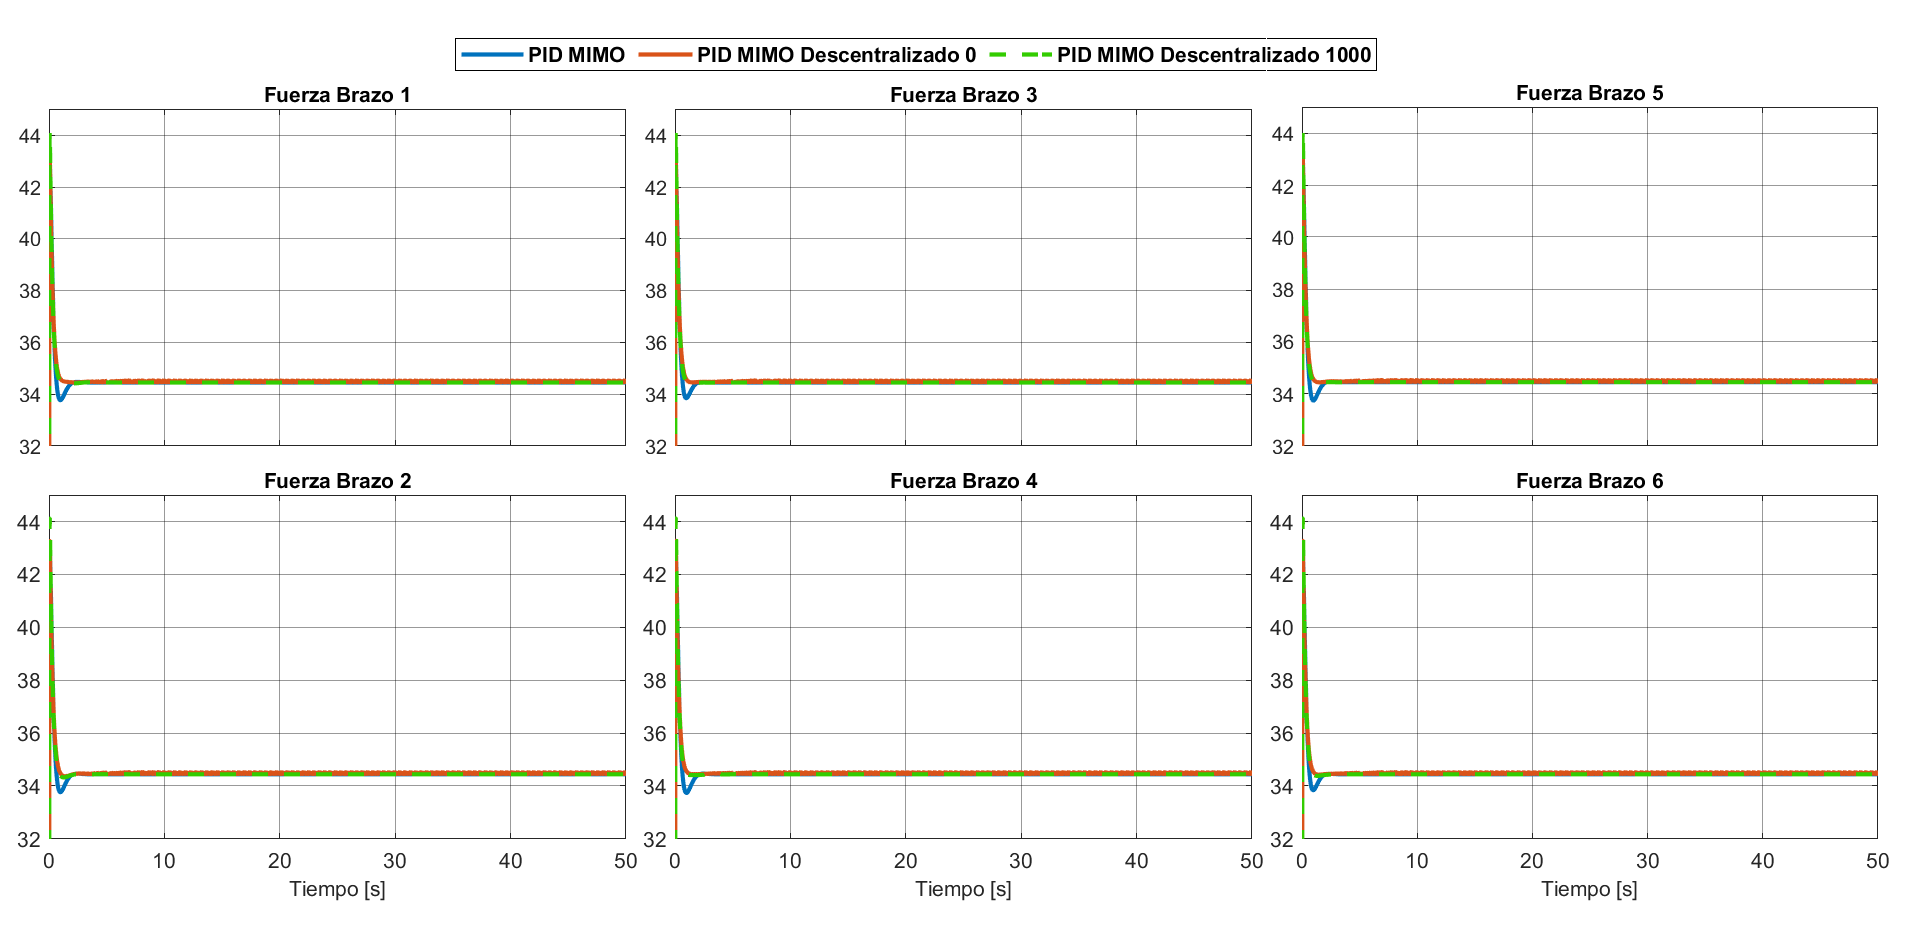
\includegraphics[width=1\columnwidth]{Results/mimoPID_escalon/CASO_2_fuerza_escalon.eps}
    \caption{CASO 2 Fuerza de actuación (N), referencia escalón.}
    \label{fig:result_mimoPID_escalon_fuerza2}
\end{figure}

Finalmente es posible deducir, que los valores de $Q$ y $R$ influyen considerablemente en la estabilidad de la plataforma Stewart, más específicamente en los controladores descentralizados analizados. Para valores de respuesta de control lenta, los controladores descentralizados normal y optimizado no son capaces de estabilizar la planta. Por lo tanto debido a los resultados, el controlador MIMO PID Full logra ser el más completo de todos, ya que posee los mejores índices de desempeño, no presenta desestabilizaciones, y garantiza además error cero en estado estacionario, para señales de referencia de tipo escalón.

%%%%%%%%%%%%%%%%%%%%%%%%%%%%%%%%%%%%%%%%%%%%%%%%
\subsection{Referencia Sinusoidal Nro 1 (caso estable)}

Se establece la señal de referencia para el movimiento de la plataforma superior, compuesta por señales de tipo sinusoidales:
\begin{equation} 
    q_{ref} = \begin{bmatrix}
        0 & 0 & 12+3sin(\pi t) & 0 & 0 & 15sin(\pi t)
    \end{bmatrix}^{\top}
\end{equation}

\begin{remark}
En el modelo Simulink de la simulación se asigna la referencia en grados (se posee un bloque interno de conversor de grados a radianes).
\end{remark}

Para un tiempo de simulación de $T_{sim}=50(s)$ se obtienen los resultados de los índices de desempeño mostrados en la tabla comparativa \ref{tab:indices_mimopid_sinusoidal_nro1}.

\begin{table}[ht]
\centering
\begin{tabular}{c|c|c|c|c|}
\cline{2-5}
    & \textbf{PID MIMO} & $\mathbf{J_{ISE}}$ & $\mathbf{J_{u}}(\cdot10^5)$ & $\mathbf{J_{LQI}}(\cdot10^6)$ \\ \hline
\multicolumn{1}{|c|}{\multirow{3}{*}{Caso 1}} &  Full               & $3455$ & $3.6281$ & $0.3468$ \\ \cline{2-5} 
\multicolumn{1}{|c|}{}                        & Descentralizado 0   & $4230$ & $3.6494$ & $1.1250$ \\ \cline{2-5} 
\multicolumn{1}{|c|}{}                        & Descentralizado 1000& $3959$ & $3.6444$ & $0.9164$ \\ \hline
\multicolumn{1}{|c|}{\multirow{3}{*}{Caso 2}} & Full                & $2584$ & $3.7691$ & $1.3043$ \\ \cline{2-5} 
\multicolumn{1}{|c|}{}                        & Descentralizado 0   & $2465$ & $3.8132$ & $2.7398$ \\ \cline{2-5} 
\multicolumn{1}{|c|}{}                        & Descentralizado 1000& $2416$ & $3.8533$ & $2.5489$ \\ \hline
\end{tabular}
\caption{Desempeño para PID MIMO Full y PID MIMO Descentralizado con $N=0$ y $N=1000$ iteraciones, referencia sinusoidal Nro 1.}
\label{tab:indices_mimopid_sinusoidal_nro1}
\end{table}

De la tabla \ref{tab:indices_mimopid_sinusoidal_nro1} podemos notar los altos valores del índice $J_{ISE}$ para todos los controladores, debido a la incapacidad de los 3 controladores de seguir a la referencia sinusoidal número 1. Debido a esto, es que este índice $J_{ISE}$ no sigue el mismo comportamiento del caso de la referencia escalón. De acá, se aprecia que el controlador MIMO PID Descentralizado 1000 posee mejor rendimiento que su versión descentralizada no optimizada.

Por otro lado para el índice de esfuerzo de control $J_u$, si tomamos como referencia el controlador MIMO PID Full, el controlador MIMO PID Descentralizado 0 presenta un incremento del $0.5\%$ para el Caso 1 y un $1.17\%$ para el Caso 2. El controlador óptimo MIMO Descentralizado 1000 posee un incremento del $0.4\%$ para el Caso 1 y un $2.2\%$ para el Caso 2. Esto nos dice que el controlador MIMO PID Full necesita de un esfuerzo de control menor para controlar el sistema, siendo mejor que las versiones descentralizadas en este ámbito.

Finalmente para el funcional de costo $J_{LQI}$ notamos que el controlador MIMO PID Full minimiza de mejor manera en comparación a sus versiones descentralizadas. Tomando como referencia el controlador MIMO PID Full se puede notar que el controlador MIMO PID Descentralizado 0 posee un incremento del índice $J_{LQI}$ del $224\%$ para el Caso 1 y un $110\%$ para el Caso 2. Para el controlador optimizado MIMO PID Descentralizado 1000 se posee un incremento del $164\%$ para el Caso 1 y un $95\%$ para el Caso 2.

Con estos índices analizados, se podría decir que el controlador MIMO PID Full es la mejor opción en la mayoría de los índices de desempeño para la referencia sinusoidal número 1. Aun así, en el caso 2 se presenta una anomalía donde el controlador optimizado descentralizado 1000 presenta mejor desempeño en el índice $J_{ISE}$ que el controlador MIMO PID Full, que posiblemente sea por la incapacidad de seguir de forma adecuada a la señal sinusoidal número 1. Puede darse el caso de que al cambiar la frecuencia, el MIMO PID Full sea mejor en el índice $J_{ISE}$, pero como se menciono, debido a la incapacidad del diseño de control de seguir a referencias sinusoidales es que da lugar a que se presenten estas anomalías.

En las Figuras \ref{fig:result_mimoPID_sinusoidal_nro1_error1} y \ref{fig:result_mimoPID_sinusoidal_nro1_fuerza1} se muestra el error de seguimiento y la fuerza aplicada respectivamente en cada brazo del sistema para el Caso 1. 

Con los $Q$ y $R$ escogidos para el Caso 1, caracterizándose por establecer una velocidad de control un poco más lenta, podemos notar que las versiones descentralizadas del controlador poseen un transciente más extenso, debido a la falta de sus elementos fuera de la diagonal que aportan en el control del sistema. Por otro lado, debido a la incapacidad de todos los controladores de seguir a la referencia sinusoidal Nro.1, es que se poseen magnitudes elevadas del error en estado estacionario.
    
\begin{figure}[H]
\centering
    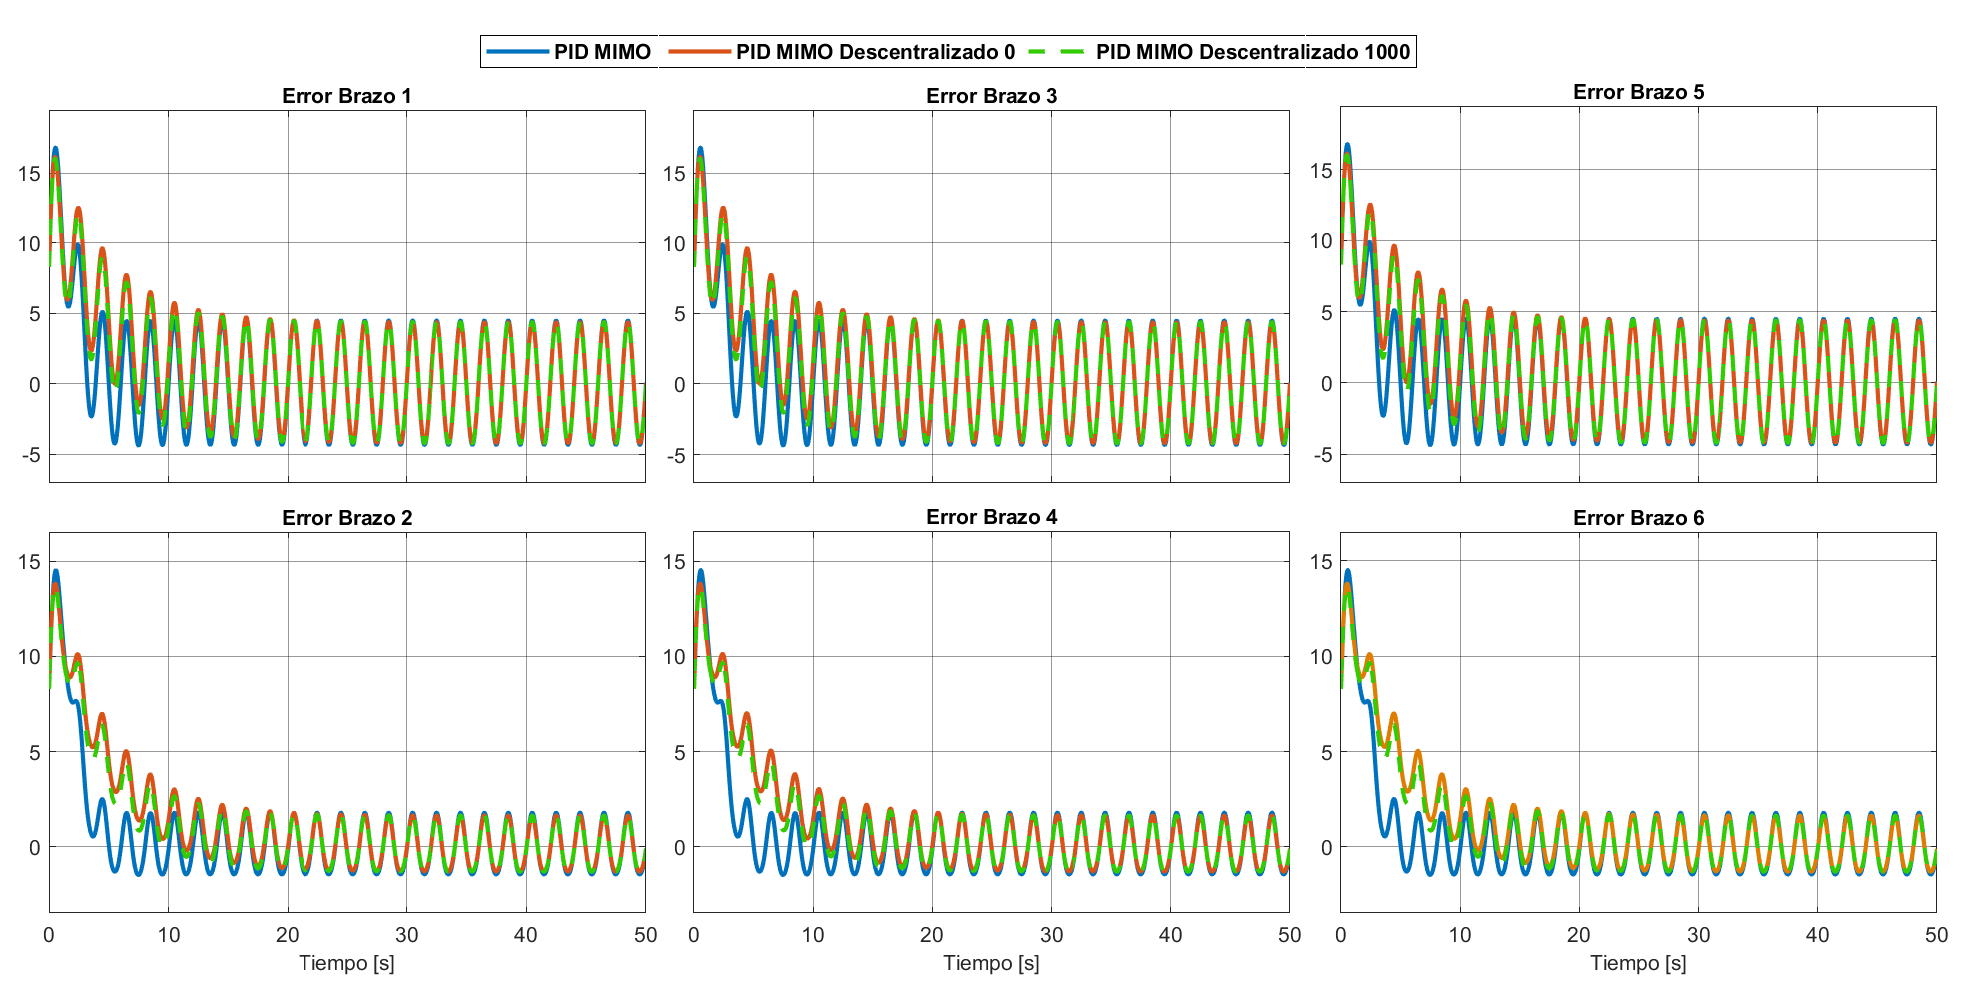
\includegraphics[width=1\columnwidth]{Results/mimoPID_sinusoidal/CASO_1_error_sinusoidal.eps}
    \caption{CASO 1 Error de seguimiento (cm), referencia sinusoidal Nro 1.}
    \label{fig:result_mimoPID_sinusoidal_nro1_error1}
\end{figure}

\begin{figure}[H]
\centering
    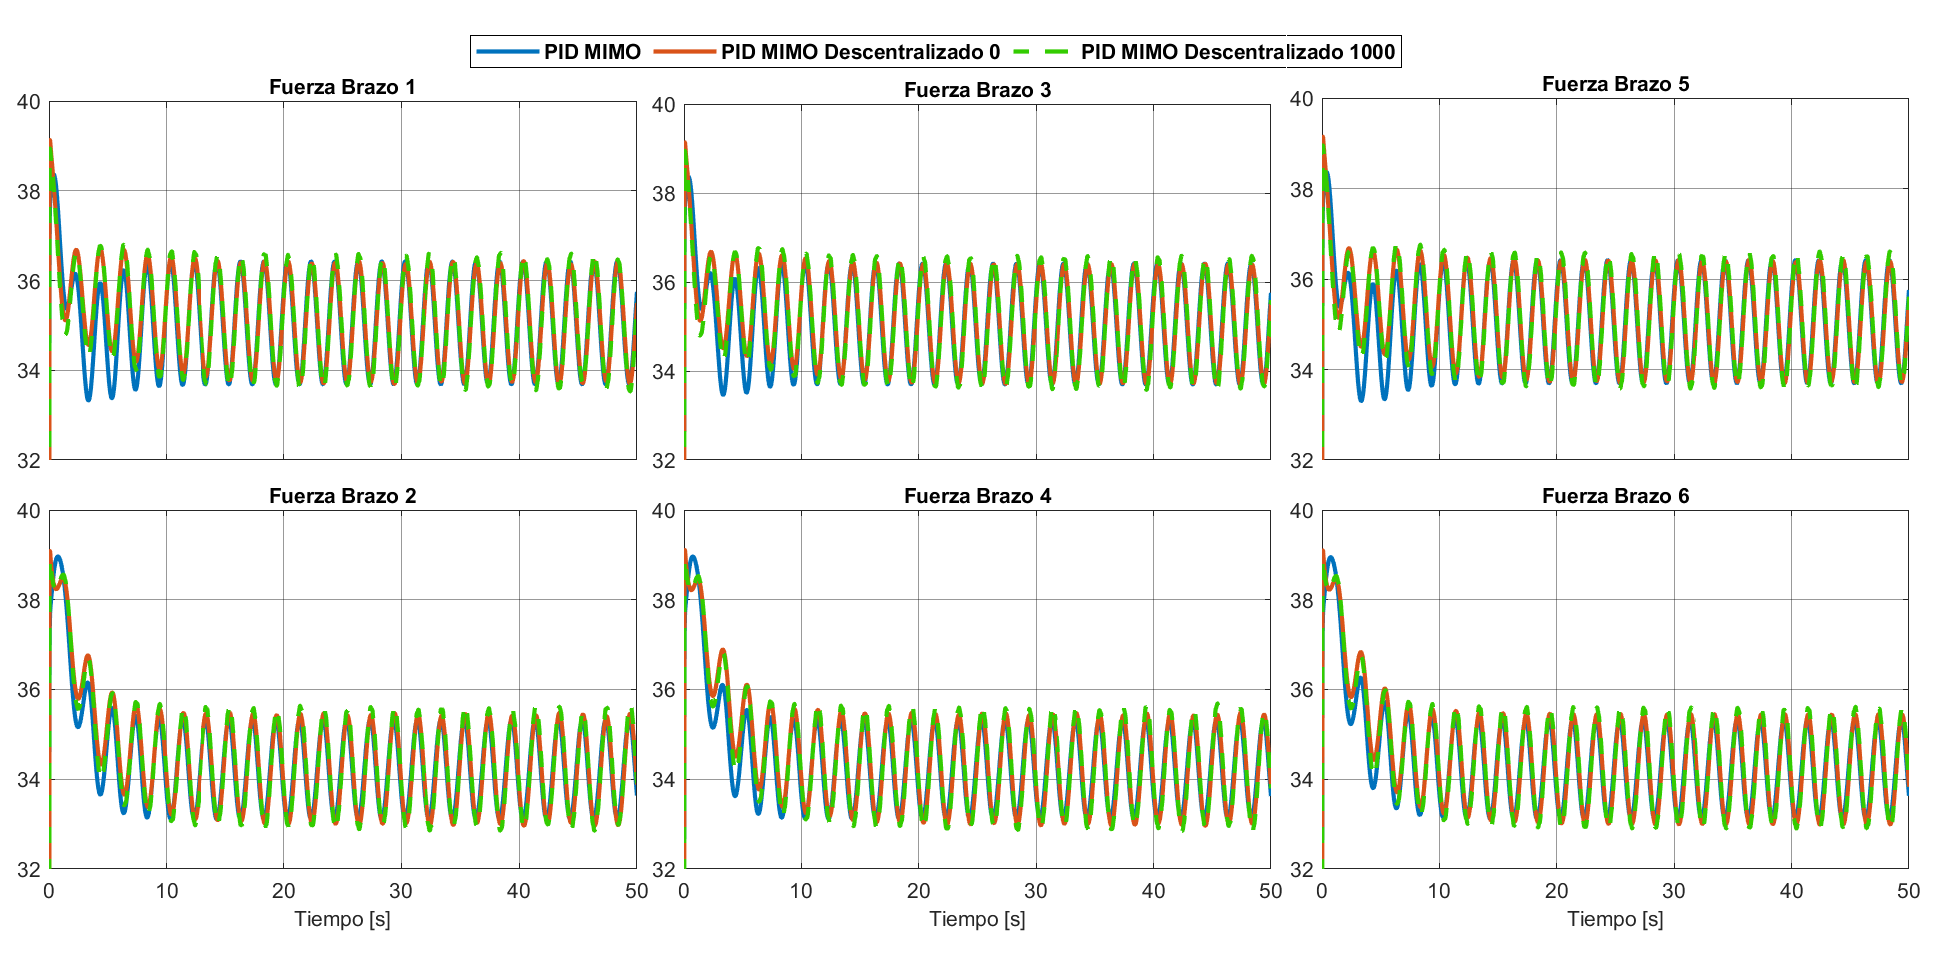
\includegraphics[width=1\columnwidth]{Results/mimoPID_sinusoidal/CASO_1_fuerza_sinusoidal.eps}
    \caption{CASO 1 Fuerza de actuación (N), referencia sinusoidal Nro 1.}
    \label{fig:result_mimoPID_sinusoidal_nro1_fuerza1}
\end{figure}

Para el Caso 2, al cambiar las matrices $Q$ y $R$ logrando una velocidad más rápida del control, seguimos notando altos valores de error y de fuerza aplicada al sistema. En las Figuras \ref{fig:result_mimoPID_sinusoidal_nro1_error2} y \ref{fig:result_mimoPID_sinusoidal_nro1_fuerza2} se muestra el error de seguimiento y la fuerza aplicada respectivamente en cada brazo de la plataforma. 

\begin{figure}[H]
\centering
    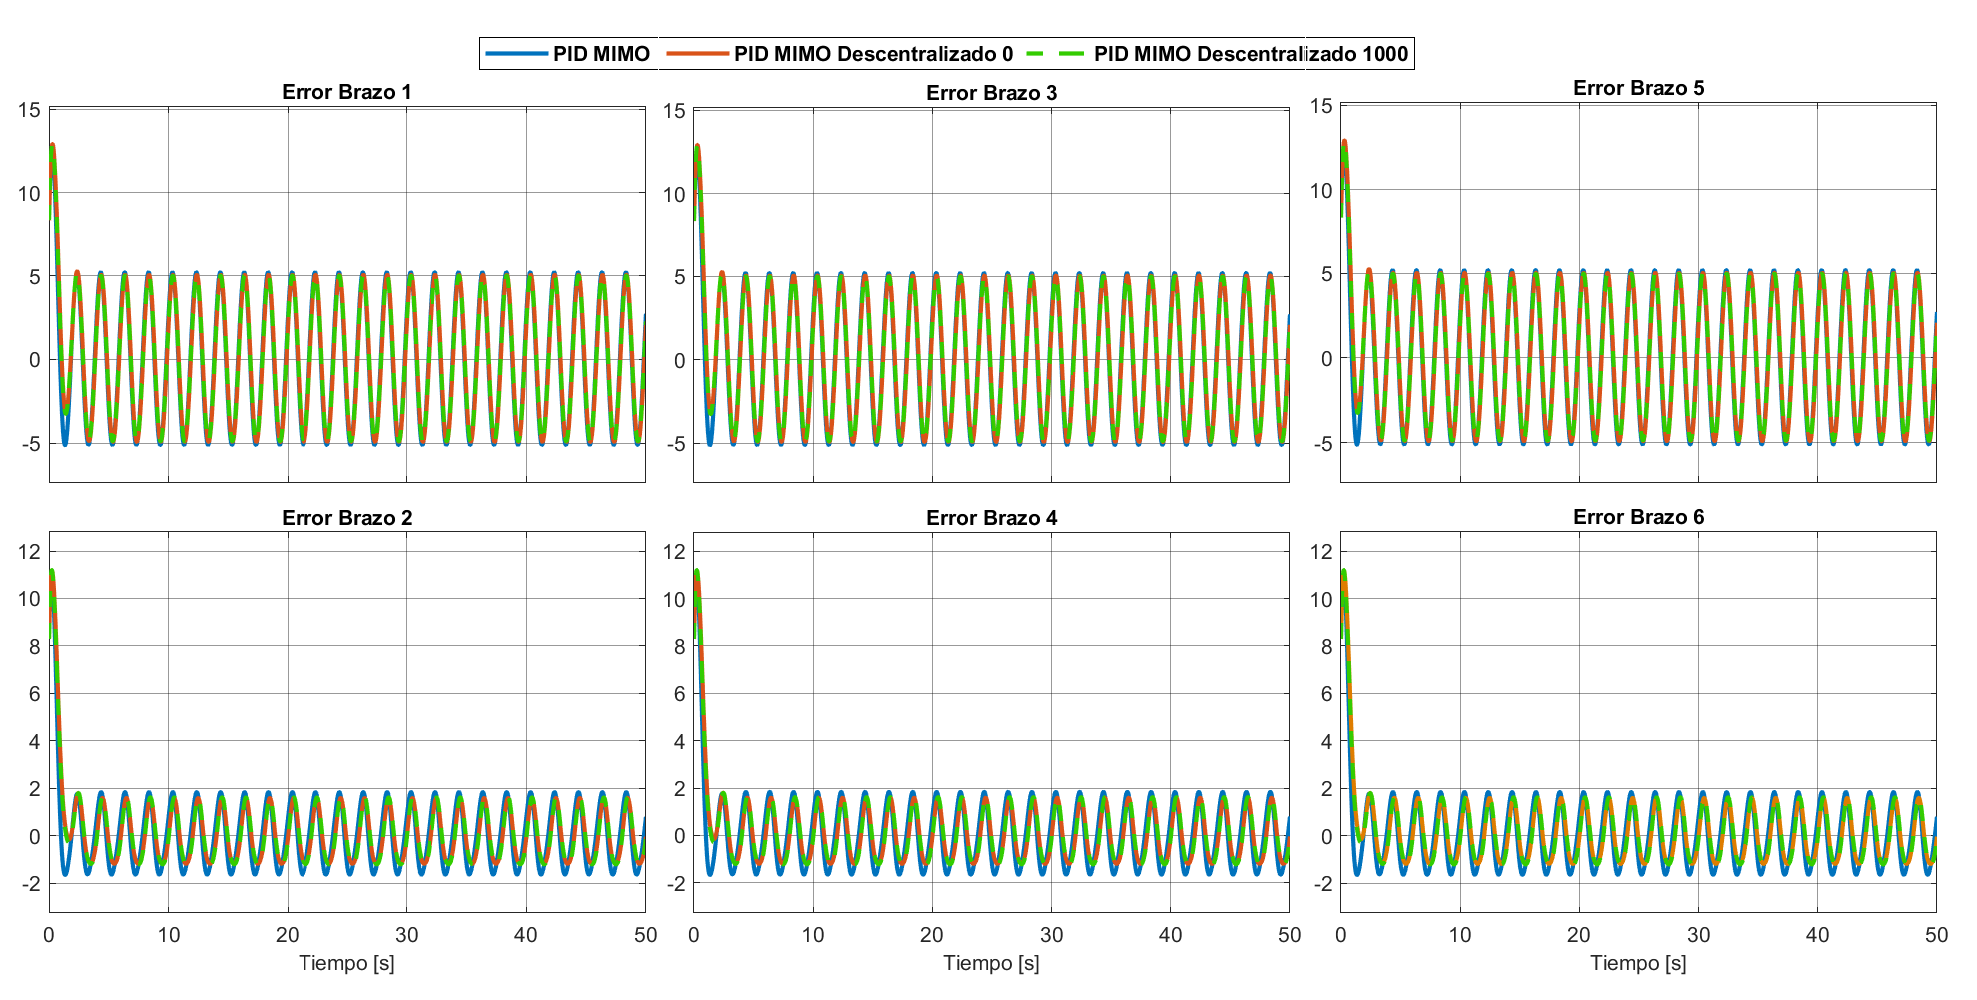
\includegraphics[width=1\columnwidth]{Results/mimoPID_sinusoidal/CASO_2_error_sinusoidal.eps}
    \caption{CASO 2 Error de seguimiento (cm), referencia sinusoidal Nro 1.}
    \label{fig:result_mimoPID_sinusoidal_nro1_error2}
\end{figure}

\begin{figure}[H]
\centering
    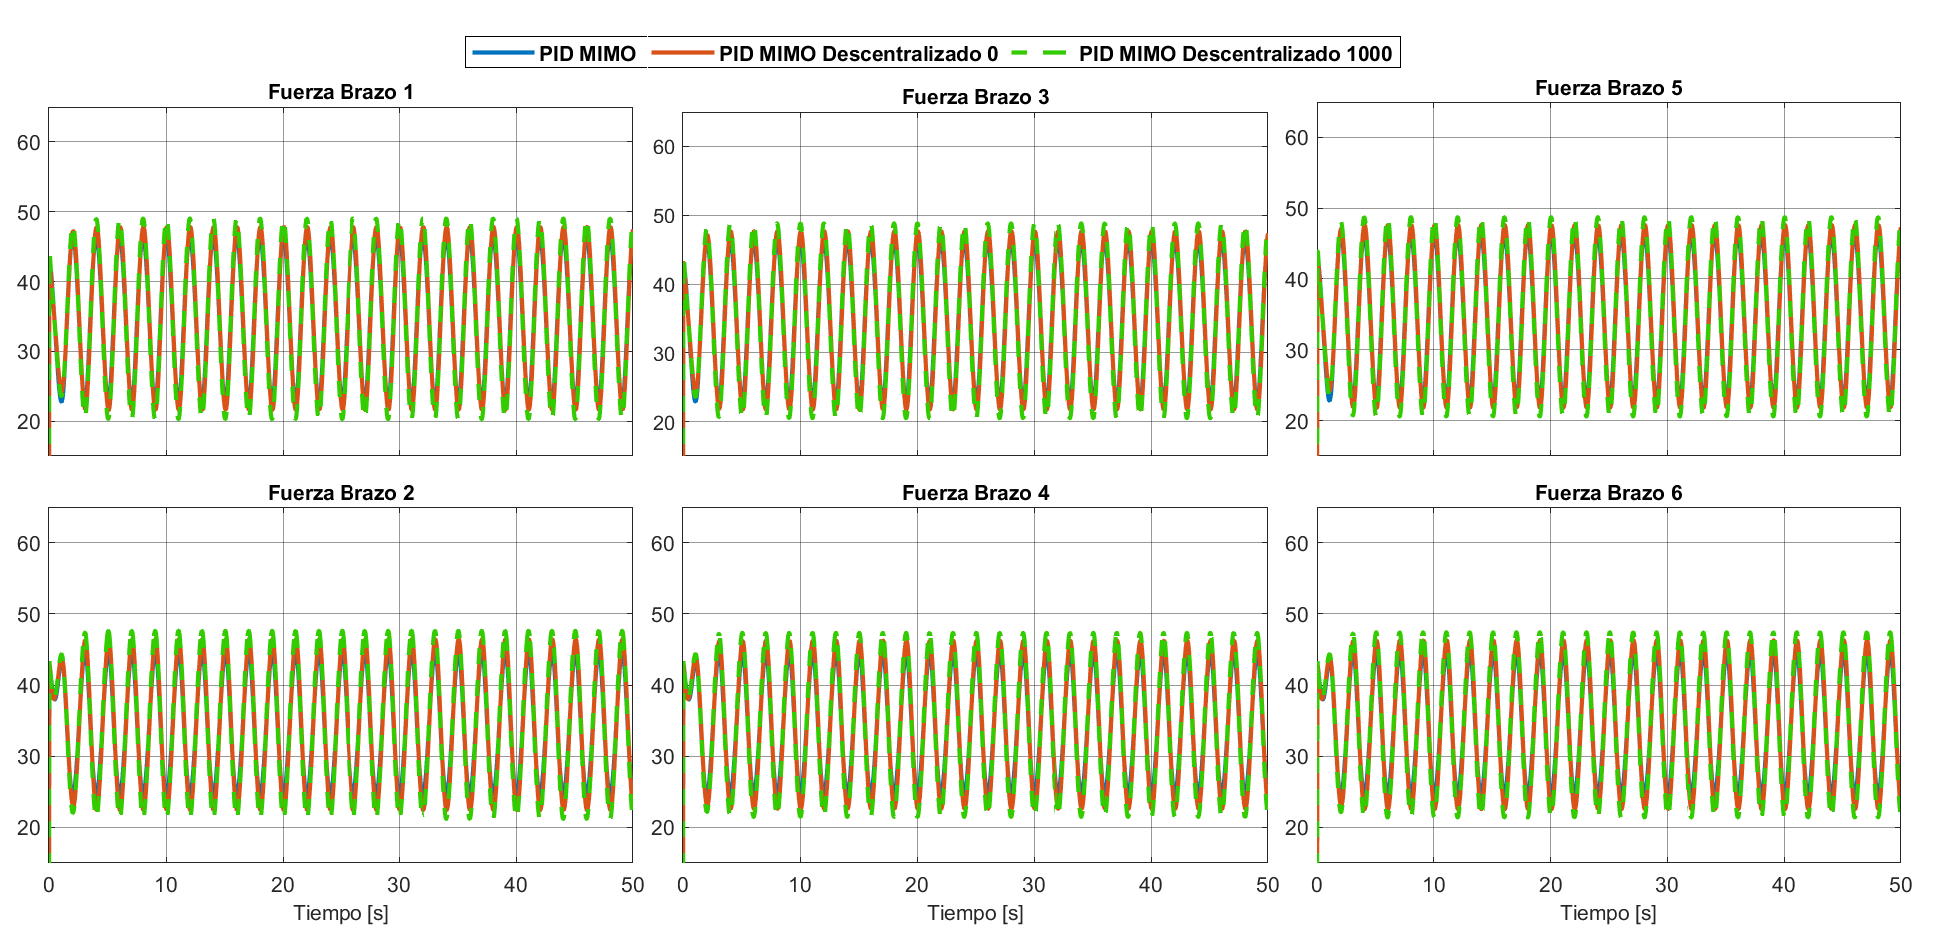
\includegraphics[width=1\columnwidth]{Results/mimoPID_sinusoidal/CASO_2_fuerza_sinusoidal.eps}
    \caption{CASO 2 Fuerza de actuación (N), referencia sinusoidal Nro 1.}
    \label{fig:result_mimoPID_sinusoidal_nro1_fuerza2}
\end{figure}

Por lo tanto, es posible deducir que independiente del valor de $Q$ y $R$ que uno asigne al control, ya sea para aumentar la velocidad de control, no se podrá obtener un seguimiento perfecto a la señal sinusoidal número 1. Esto se evidencia con los altos índices de desempeño analizados y las gráficas de error y de fuerza con sus valores elevados. Se debe notar que el sistema en ningún momento se desestabiliza, es capaz de garantizar cierta estabilidad en el control, pero sin poder garantizar un error de seguimiento cero en estado estacionario.

%%%%%%%%%%%%%%%%%%%%%%%%%%%%%%%%%%%%%%%%%%%%%%%%
\subsection{Referencia Sinusoidal Nro 2 (caso inestable)}

Se establece una segunda señal de referencia de tipo sinusoidal para la plataforma superior, siendo levemente más compleja que la referencia sinusoidal Nro 1, ya que genera un movimiento sinusoidal diferente en cada brazo (diferencias en frecuencia, fase y/o amplitud):

\begin{equation} 
    q_{ref} = \begin{bmatrix}
        0 & 0 & 12+3sin(\pi t) & 10sin(\pi t) & 10sin\left(\pi t - \frac{\pi}{2}\right) & 0
    \end{bmatrix}^{\top}
\end{equation}

\begin{remark}
    En el modelo Simulink de la simulación se asigna la referencia en grados (se posee un bloque interno de conversor de grados a radianes).
\end{remark}

Para un tiempo de simulación de $T_{sim}=50(s)$ se obtienen los resultados de los índices de desempeño mostrados en la tabla comparativa \ref{tab:indices_mimopid_sinusoidal_nro2}.

\begin{table}[ht]
\centering
\begin{tabular}{c|c|c|c|c|}
\cline{2-5}
    & \textbf{PID MIMO} & $\mathbf{J_{ISE}}$ & $\mathbf{J_{u}}(\cdot10^5)$ & $\mathbf{J_{LQI}}(\cdot10^6)$ \\ \hline
\multicolumn{1}{|c|}{\multirow{3}{*}{Caso 1}} &  Full               & $4377$ & $3.6146$ & $0.3794$ \\ \cline{2-5} 
\multicolumn{1}{|c|}{}                        & Descentralizado 0   & $5331$ & $3.6597$ & $1.2664$ \\ \cline{2-5} 
\multicolumn{1}{|c|}{}                        & Descentralizado 1000& $5080$ & $3.7534$ & $1.0319$ \\ \hline
\multicolumn{1}{|c|}{\multirow{3}{*}{Caso 2}} & Full                & $3721$ & $4.4391$ & $1.4834$ \\ \cline{2-5} 
\multicolumn{1}{|c|}{}                        & Descentralizado 0   & $6821$ & $15.362$ & $2.9544$ \\ \cline{2-5} 
\multicolumn{1}{|c|}{}                        & Descentralizado 1000& $3770$ & $9.6146$ & $1.9650$ \\ \hline
\end{tabular}
\caption{Desempeño para PID MIMO Full y PID MIMO Descentralizado con $N=0$ y $N=1000$ iteraciones, referencia sinusoidal Nro 2.}
\label{tab:indices_mimopid_sinusoidal_nro2}
\end{table}

De la tabla \ref{tab:indices_mimopid_sinusoidal_nro2}, al igual que para la referencia de tipo escalón y tipo sinusoidal número 1, el controlador MIMO PID Full posee los mejores índices de desempeño para ambos casos analizados. 

Para el índice del error cuadrático $J_{ISE}$, si tomamos como referencia el controlador MIMO PID Full podemos hacer una comparativa porcentual con sus versiones descentralizadas. El controlador MIMO PID Descentralizado 0 posee un incremento del $J_{ISE}$ del $21.7\%$ para el Caso 1 y un $83.3\%$ para el Caso 2. El controlador optimizado MIMO PID Descentralizado 1000 posee un aumento del $16\%$ en el Caso 1 y un $1.3\%$ en el Caso 2.

Si en el esfuerzo de control $J_u$ tomamos como referencia el controlador MIMO PID Full, notamos que el controlador MIMO PID Descentralizado 0 posee un incremento de $1.2\%$ para el Caso 1 y un $246\%$ para el Caso 2. Para el controlador optimizado MIMO PID Descentralizado 1000 se obtiene un aumento del $3.8\%$ en el Caso 1 y un $116\%$ en el Caso 2, evidenciándose la inestabilidad de las versiones descentralizadas en el Caso 2.

Finalmente al analizar el funcional de costo $J_{LQI}$ la versión MIMO PID Full del controlador es la que mejor minimiza el funcional. Tomando este controlador como referencia, notamos que el controlador MIMO PID Descentralizado 0 posee un incremento del $233\%$ en el Caso 1 y un $99\%$ en el Caso 2. Para el controlador optimizado MIMO PID Descentralizado 1000 se posee un aumento del $171\%$ para el Caso 1 y un $32.4\%$ para el Caso 2.

Por esto, el controlador MIMO PID Full es el mejor al tener menor error cuadrático $J_{ISE}$, un menor esfuerzo de control $J_u$ y un funcional de coste menor $J_{LQI}$. El algoritmo de optimización logra mejorar los índices del controlador descentralizado, pero aun así, no es capaz de igualar el rendimiento del controlador MIMO PID Full con la referencia sinusoidal número 2.

En las Figuras \ref{fig:result_mimoPID_sinusoidal_nro2_error1} y \ref{fig:result_mimoPID_sinusoidal_nro2_fuerza1} correspondientes al Caso 1, se pueden apreciar los errores de seguimiento y la fuerza de la actuación respectivamente de cada brazo de la plataforma Stewart. El controlador MIMO PID es el único de los 3 controladores que no se desestabiliza, sin embargo posee altos valores de error de seguimiento. Por otro lado, los controladores descentralizados además de poseer valores altos de error de seguimiento, son inestables con el sistema, mostrándose una fuerza de actuación descontrolada a partir de los 30 segundos en adelante. 

\begin{figure}[H]
\centering
    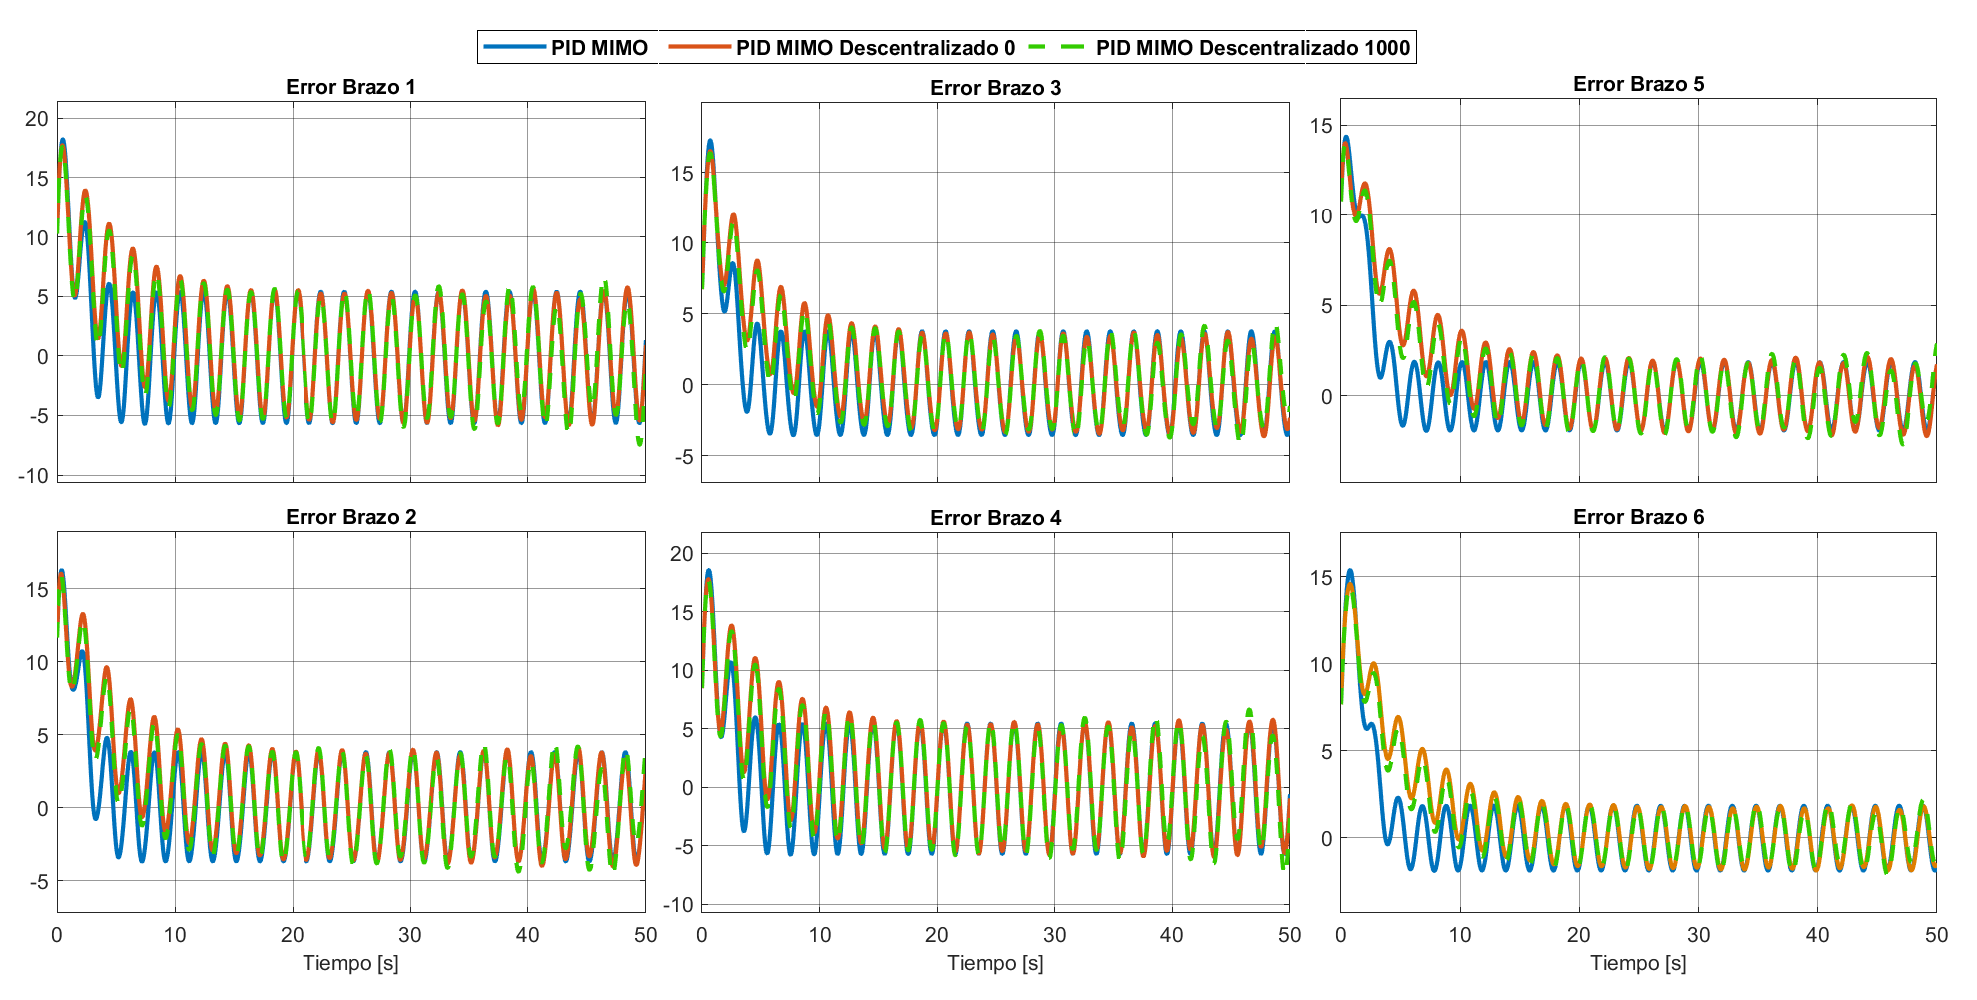
\includegraphics[width=1\columnwidth]{Results/mimoPID_sinusoidal2/CASO_1_error_sinusoidal2.eps}
    \caption{CASO 1 Error de seguimiento (cm), referencia sinusoidal Nro 2.}
    \label{fig:result_mimoPID_sinusoidal_nro2_error1}
\end{figure}
\newpage
\begin{figure}[H]
\centering
    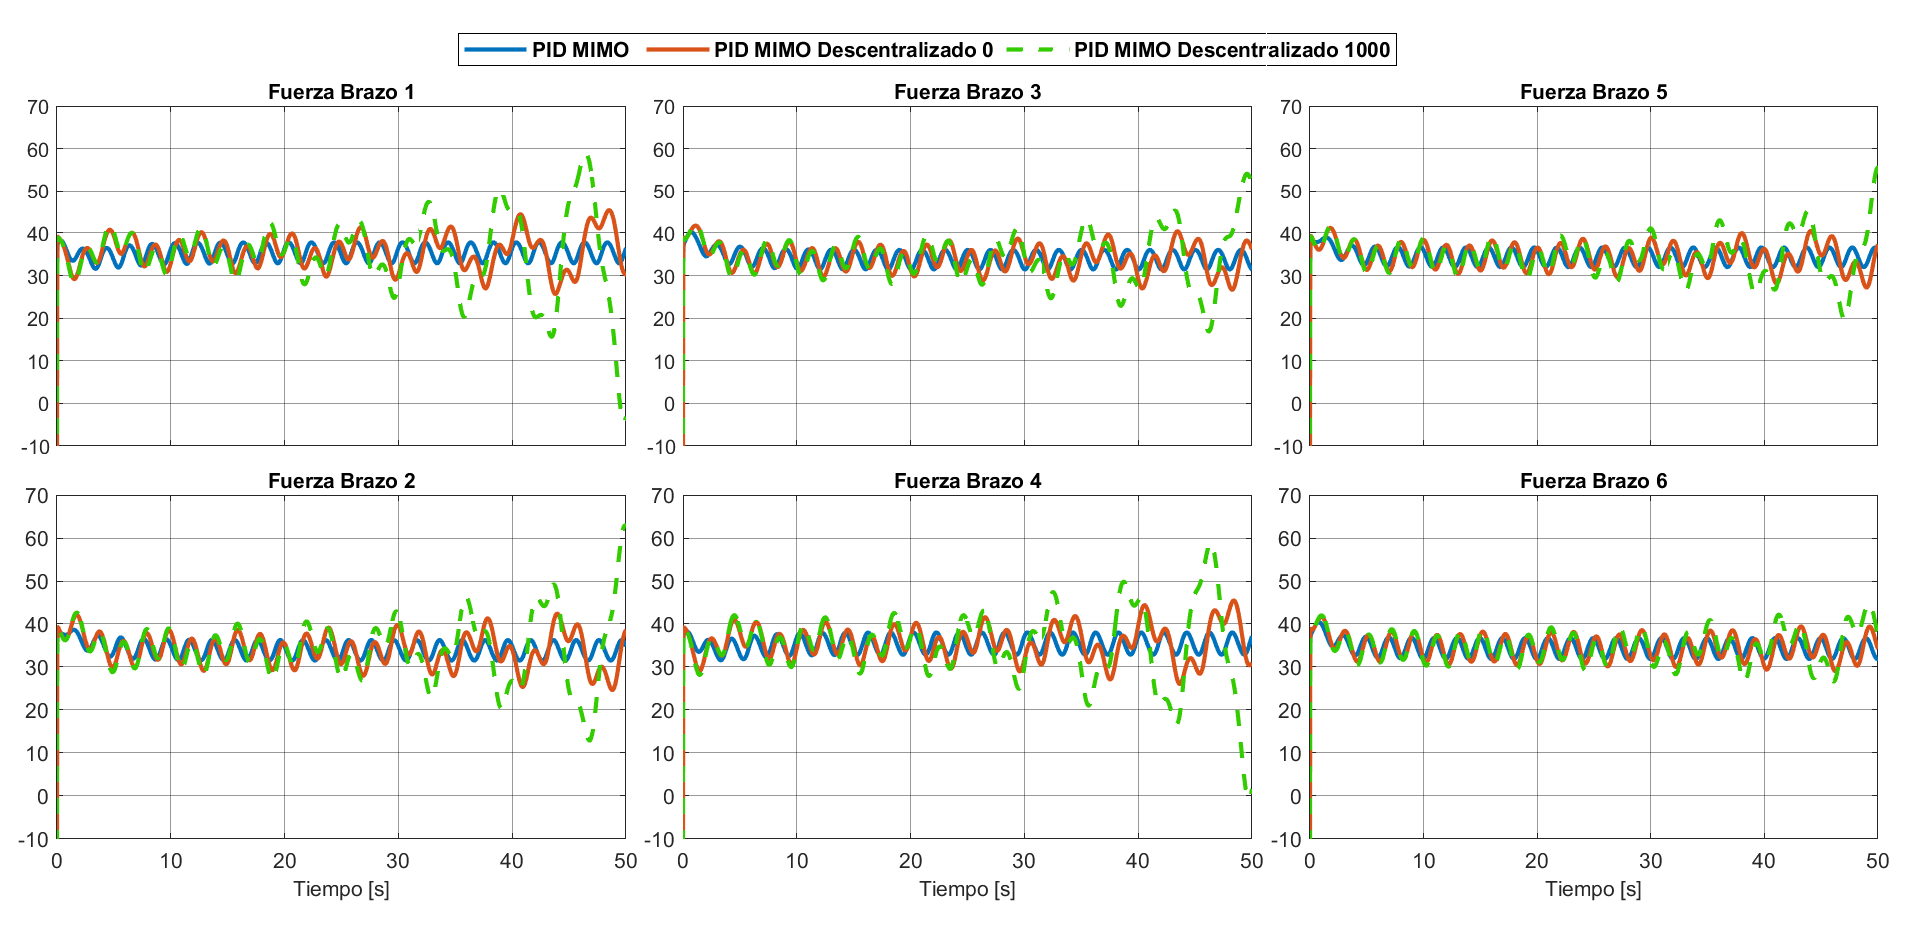
\includegraphics[width=1\columnwidth]{Results/mimoPID_sinusoidal2/CASO_1_fuerza_sinusoidal2.eps}
    \caption{CASO 1 Fuerza de actuación (N), referencia sinusoidal Nro 2.}
    \label{fig:result_mimoPID_sinusoidal_nro2_fuerza1}
\end{figure}


Para el caso 2, el cambio de las matrices $Q$ y $R$ no mejoran la respuesta del sistema ante la señal de referencia sinusoidal número 2. En las Figuras \ref{fig:result_mimoPID_sinusoidal_nro2_error2} y \ref{fig:result_mimoPID_sinusoidal_nro2_fuerza2} se muestran los errores de seguimiento y fuerzas de actuación de los brazos para el Caso 2. Los 3 controladores analizados poseen altos valores de error y de actuación, además de presentar una evidente inestabilidad en todas las gráficas con los controladores descentralizados. 

\begin{figure}[H]
\centering
    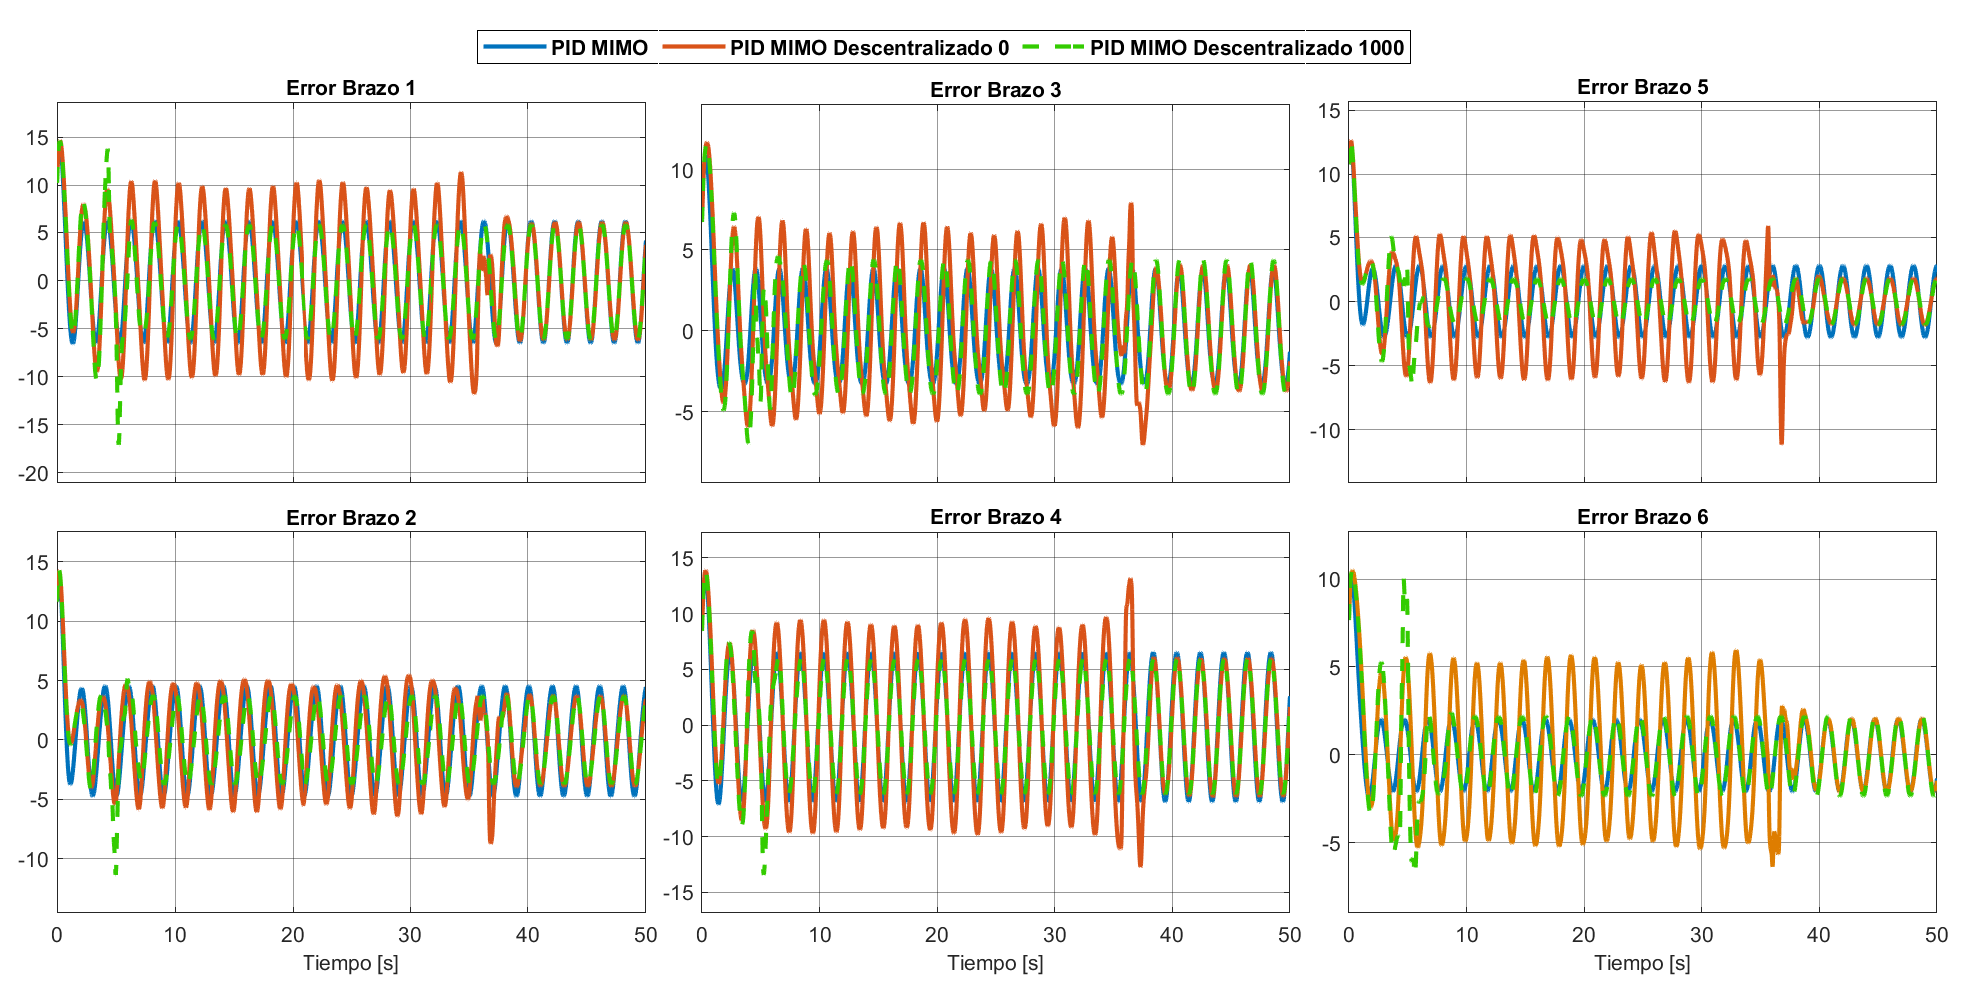
\includegraphics[width=1\columnwidth]{Results/mimoPID_sinusoidal2/CASO_2_error_sinusoidal2.eps}
    \caption{CASO 2 Error de seguimiento (cm), referencia sinusoidal Nro 2.}
    \label{fig:result_mimoPID_sinusoidal_nro2_error2}
\end{figure}

\begin{figure}[H]
\centering
    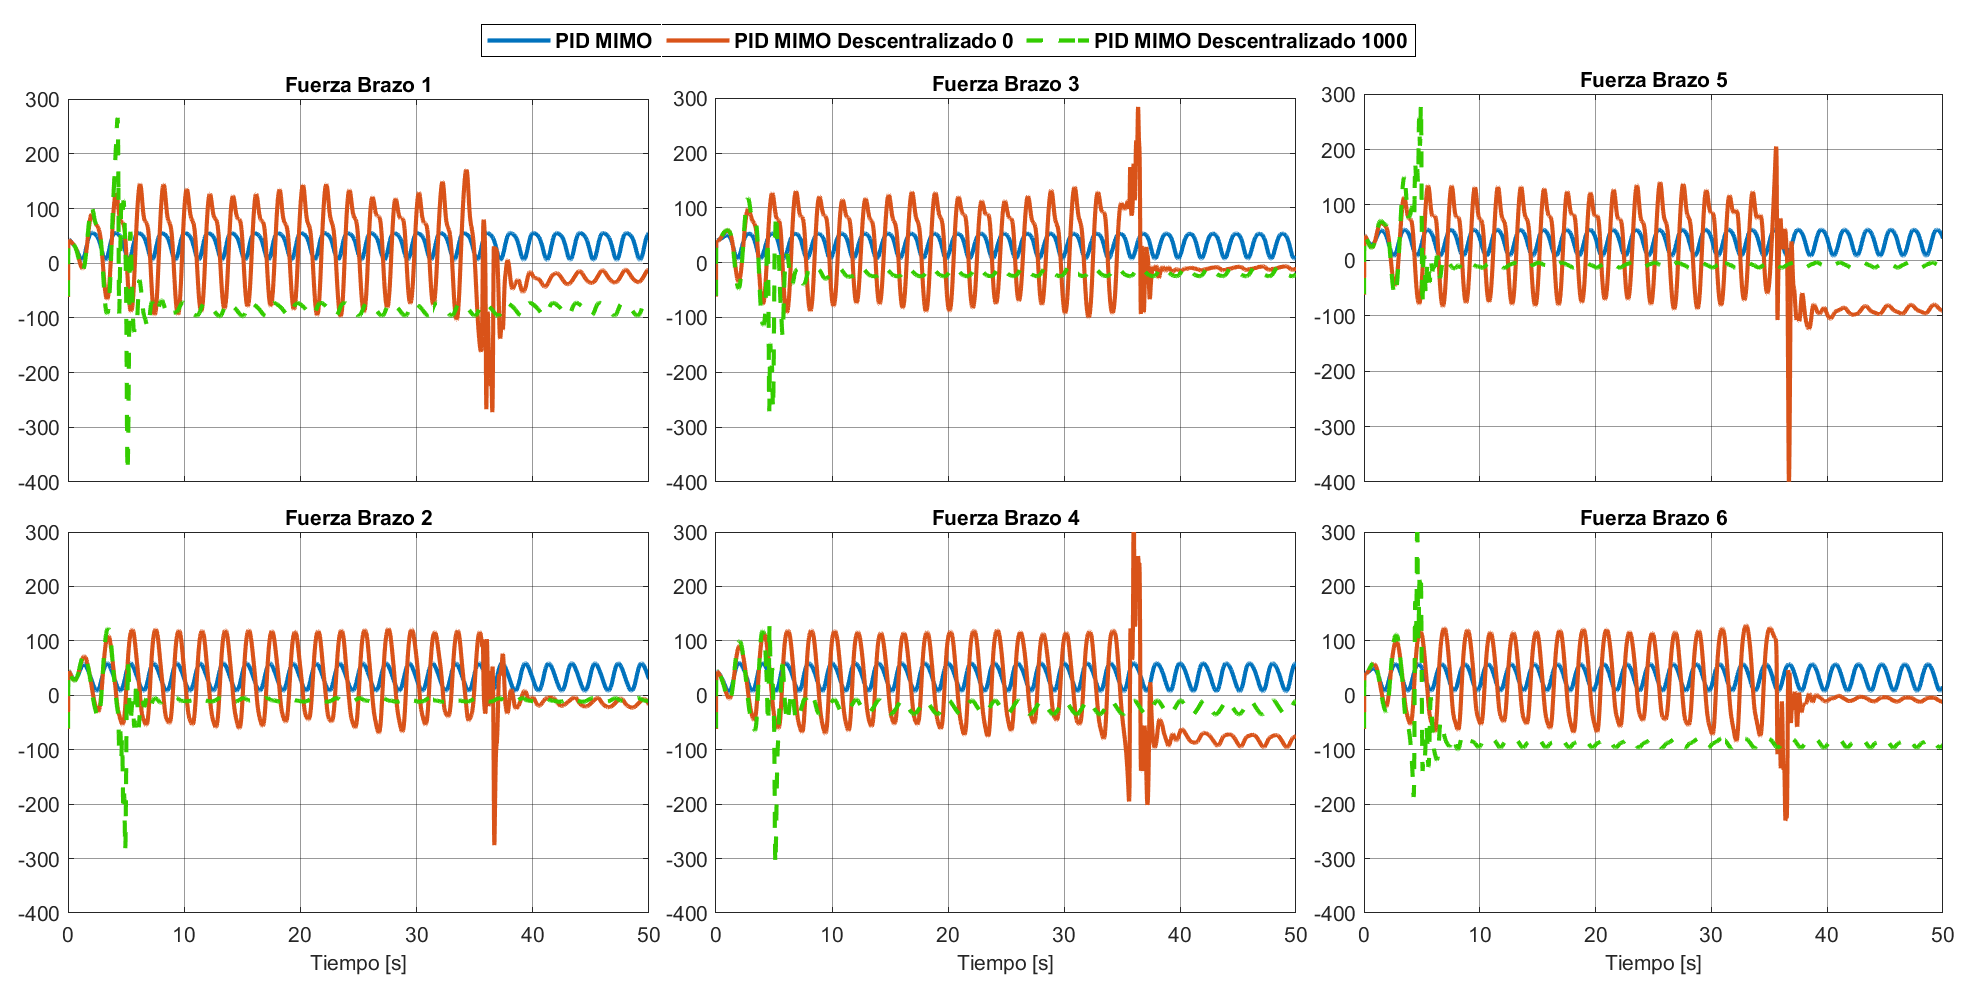
\includegraphics[width=1\columnwidth]{Results/mimoPID_sinusoidal2/CASO_2_fuerza_sinusoidal2.eps}
    \caption{CASO 2 Fuerza de actuación (N), referencia sinusoidal Nro 2.}
    \label{fig:result_mimoPID_sinusoidal_nro2_fuerza2}
\end{figure}

Finalmente es posible deducir, que ante señales de tipo sinusoidales los controladores MIMO PID analizados (full y descentralizados) no son eficientes. Todos ellos presentan altas magnitudes de error de seguimiento, además de inestabilidad por parte de los controladores descentralizados. La ventaja principal del controlador MIMO PID Full con los demás, es que logra garantizar una estabilidad del sistema, además de presentar mejores índices de desempeño en comparación a sus versiones descentralizadas (normal y optimizada), debido a la presencia de los elementos fuera de la diagonal de la matriz de control, pero con el inconveniente de presentar un desempeño claramente deficiente ante referencias sinusoidales\\

Por lo tanto, el diseño de control MIMO PID sintetizado mediante un control LQI no garantiza error de seguimiento cero en estado estacionario para señales de referencia de tipo sinusoidal. Para solucionar esto, en el capítulo \ref{cap:OutputRegulation} siguiente, se diseña un control que garantice un seguimiento eficiente de referencias de señales sinusoidales en estado estacionario.

